%% =====================================================================
%% MDPI Processes — Article Template (production-ready)
%% Autor: Bryan Salas — Universidad Nacional de Colombia, Sede La Paz
%% Versión: comparación de 4 controladores con validación estadística N=4
%% =====================================================================
%%
%% COMPILACIÓN EN OVERLEAF:
%%   1. New Project > From Template > MDPI Article Template (Processes).
%%   2. Reemplazar el .tex de ejemplo por este archivo.
%%   3. Crear la carpeta `figuras_articulo/` y subir los PNG generados por
%%      trainv2/generar_figuras.py, generar_figuras_4ctrl.py y
%%      generar_figuras_setpoint.py.
%%   4. Compilar con pdfLaTeX.
%% =====================================================================
\documentclass[processes,article,submit,moreauthors,pdftex]{Definitions/mdpi}

% ── Paquetes ─────────────────────────────────────────────────
\usepackage{booktabs}
\usepackage{multirow}
\usepackage{amsmath,amssymb,amsthm}
\usepackage{graphicx}
\usepackage{siunitx}
\usepackage{subcaption}
\usepackage{algorithm}
\usepackage{algpseudocode}
\usepackage{xcolor}
\usepackage{tabularx}
\usepackage{array}
% NOTA: la clase MDPI ya carga hyperref; no se vuelve a cargar aquí.

% ── Comandos de conveniencia ─────────────────────────────────
\newcommand{\Qu}{Q_u}
\newcommand{\Tref}{T^*}
\newcommand{\Tobs}{T_{\mathrm{obs}}}
\newcommand{\eT}{e_T}
\newcommand{\dt}{\Delta t}
\DeclareMathOperator*{\argmin}{arg\,min}

% ── Compatibilidad entre versiones de la clase MDPI ──────────
% La clase de 2020 no define estos comandos (sí las versiones nuevas
% de Overleaf). \providecommand sólo los crea si aún no existen.
\providecommand{\TitleCitation}[1]{}
\providecommand{\dataavailability}[1]{%
  \par\medskip\noindent\textbf{Data Availability Statement:} #1}
\providecommand{\doi}[1]{doi:\,#1}
\AtBeginDocument{\hypersetup{hidelinks}}

% ── Idioma: etiquetas en español ─────────────────────────────
% La clase MDPI hereda «Figure»/«Table» del article base; se fuerzan
% al español. El título de la bibliografía se fija con \reftitle.
\AtBeginDocument{%
  \renewcommand{\figurename}{Figura}%
  \renewcommand{\tablename}{Tabla}%
}
\reftitle{Referencias}

\graphicspath{{figuras/}{figuras_articulo/}}

% ── Metadatos ────────────────────────────────────────────────
\Title{Control Robusto de Temperatura en Plantas Térmicas FOPDT
con Tiempos Muertos Dinámicos Masivos Mediante un Agente
Soft Actor-Critic Entrenado con Curriculum Learning: Validación
Empírica en Hardware Real}

\TitleCitation{Control Térmico Robusto con SAC y Curriculum Learning}

\Author{Bryan José Salas Altahona\textsuperscript{1,*}}

\AuthorNames{Bryan Salas}

\address{%
  \textsuperscript{1}\quad Departamento de Ingeniería,
  Universidad Nacional de Colombia, Sede La Paz,
  La Paz, Cesar 202010, Colombia}

\corres{Correspondence: bsalas@unal.edu.co}

% ── Abstract (<=200 palabras, un párrafo, sin citas) ─────────
\abstract{%
El control de temperatura en plantas de Primer Orden con Tiempo Muerto
(FOPDT) sometidas a escalones de gran amplitud y enfriamiento asimétrico
supone un reto para los controladores clásicos y predictivos. Este artículo presenta un agente Soft Actor-Critic (SAC)
libre de modelo entrenado mediante Curriculum Learning de cuatro etapas,
con tiempos muertos dinámicos hasta \SI{33}{\second} y Domain
Randomization de $\pm 15\,\%$ sobre los parámetros físicos. El agente
(observación de 46 dimensiones, arquitectura $[64,64]$) se comparó en
hardware real (TCLab Arduino) contra tres referencias: un PI sintonizado
por IMC-Skogestad, un NMPC puro y una arquitectura híbrida residual NMPC-SAC,
bajo un perfil de estrés dinámico de \SI{600}{\second} con
cuatro fases asimétricas, replicado cuatro veces por controlador. El SAC
redujo el ISE en un $32.5\,\%$ respecto al PI (de $44{,}650$ a $30{,}137$)
y en un $32.4\,\%$ respecto al NMPC, con un sobreimpulso máximo de
$\SI{14.0}{\celsius}$ frente a $20.5$--$\SI{22.9}{\celsius}$ de las
alternativas. Las diferencias en ISE son estadísticamente significativas
(Mann-Whitney, $p=0.014$). La arquitectura híbrida NMPC-SAC resultó la
peor, por la restricción de su espacio de exploración y el efecto
escalera del solver. Las políticas libres de modelo entrenadas bajo
simulaciones estocásticas extremas superan a los métodos clásicos y
predictivos en control térmico severo.}

\keyword{Soft Actor-Critic; Curriculum Learning; control de temperatura;
FOPDT; tiempo muerto; TCLab; aprendizaje por refuerzo profundo; NMPC;
Domain Randomization; windup integral; hardware-in-the-loop}

\begin{document}

% =====================================================================
\section{Introducción}
\label{sec:intro}
% =====================================================================

El control de temperatura en procesos industriales determina la eficiencia
energética, la integridad del producto y la seguridad operacional
\cite{Seborg2016}. Muchos sistemas térmicos se modelan como plantas de
Primer Orden con Tiempo Muerto (FOPDT), descritas por la ganancia estática
$K_p$, la constante de tiempo $\tau$ y el retardo de transporte $\theta$.
De estos parámetros, el tiempo muerto es el más disruptivo, porque
introduce un retardo puro entre la acción de control y su efecto observable
e impide que un controlador realimentado anticipe las consecuencias de sus
acciones. La dificultad aumenta cuando el retardo es además variable, los
escalones de referencia son grandes y el enfriamiento es puramente pasivo,
condiciones habituales en plantas térmicas reales que este trabajo aborda
de forma explícita.

La pregunta que motiva este estudio es si una política de control libre de
modelo, entrenada únicamente en simulación bajo perturbaciones extremas,
puede superar a los controladores clásicos y predictivos al desplegarse sin
reentrenamiento en hardware real sometido a tiempos muertos largos y
variables.

\subsection{Trabajos Relacionados}
\label{subsec:related}

El control clásico aborda el tiempo muerto de dos maneras. Los reguladores
PI y PID \cite{Astrom2006} reducen su agresividad con sintonías
conservadoras, como las reglas analíticas IMC-Skogestad \cite{Skogestad2003},
a costa de respuestas lentas y de la acumulación integral o \textit{windup}
cuando el actuador satura. El Predictor de Smith \cite{Smith1957} compensa
el retardo con un modelo interno, pero su desempeño depende de la
coincidencia entre modelo y planta \cite{NormeyRico2007} y se degrada ante
variación paramétrica o no linealidades como la radiación térmica. La
plataforma de bajo costo TCLab \cite{Hedengren2019,Park2020} se ha
consolidado como banco de pruebas estándar para evaluar estas estrategias
sobre dinámicas térmicas con retardo.

El Control Predictivo No Lineal (NMPC) \cite{Rawlings2017,Mayne2014} resuelve
en cada muestreo un problema de optimización en horizonte deslizante sobre
el modelo no lineal completo, lo que le permite incorporar restricciones y
objetivos de seguimiento y energía. Su desempeño se deteriora, sin embargo,
ante perturbaciones no medidas, tiempos muertos largos o errores de modelo.
En la plataforma TCLab, Soza Mamani y Prado Romo \cite{SozaMamani2025}
reportan que el NMPC logra un seguimiento satisfactorio bajo retardos
moderados, pero que su eficacia disminuye al crecer el tiempo muerto, lo que
motiva la búsqueda de esquemas adaptativos.

El Aprendizaje por Refuerzo Profundo (DRL) \cite{Sutton2018,Mnih2015} ofrece
una vía complementaria, en la que el agente aprende una política
$\pi:\mathcal{S}\to\mathcal{A}$ por interacción con el entorno y sin modelo
explícito. En control de procesos se han aplicado el Deep Deterministic
Policy Gradient (DDPG) \cite{Lillicrap2016} y su variante Twin Delayed (TD3)
\cite{Fujimoto2018} a la regulación de temperatura en biorreactores
\cite{Rajasekhar2023} y a procesos químicos como la transesterificación
\cite{Joshi2021}, y se ha mostrado que las políticas libres de modelo
generalizan ante perturbaciones no observadas en entrenamiento
\cite{Spielberg2019,Dogru2022}. El Soft Actor-Critic (SAC) \cite{Haarnoja2018}
añade regularización por entropía, que produce políticas estocásticas más
robustas al ruido de sensores y a la incertidumbre paramétrica que las
políticas deterministas de DDPG y TD3, una propiedad valiosa frente al ruido
de cuantización del ADC de una planta física. Para explorar con seguridad las
condiciones más adversas, el Curriculum Learning \cite{Bengio2009,Narvekar2020}
expone al agente a tareas de dificultad creciente, lo que acelera la
convergencia y mejora la robustez de la política final.

Una línea reciente combina NMPC y DRL para unir la previsión del modelo con
la adaptabilidad del aprendizaje. Soza Mamani y Prado Romo \cite{SozaMamani2025}
integran agentes actor-crítico (DDPG y TD3) con NMPC sobre TCLab y concluyen
que la combinación conserva un seguimiento comparable al del NMPC y mejora la
robustez ante perturbaciones e incertidumbre de modelo. Hallazgos análogos se
reportan en el termoformado de plásticos \cite{Hosseinionari2024} y en la
climatización de edificios \cite{Chen2022}, donde la hibridación
modelo-aprendizaje mejora la adaptabilidad. Estos trabajos comparten, no
obstante, limitaciones que enmarcan la presente contribución. Su evaluación se
realiza mayormente en simulación o bajo retardos moderados, se basa en DDPG y
TD3 antes que en SAC, y no incorpora aleatorización paramétrica de la planta,
arranques en frío ni un curriculum sobre tiempos muertos dinámicos. Además,
presentan la hibridación como siempre favorable, sin contrastarla con
una política puramente libre de modelo ni cuantificar la significancia
estadística de las diferencias en hardware. En particular, ninguno documenta
que una arquitectura híbrida residual pueda resultar inferior al control libre
de modelo bajo estrés severo.

\subsection{Contribuciones}

Sobre estas limitaciones, las contribuciones de este trabajo son tres:
\begin{enumerate}
  \item Un entorno de simulación TCLab de dificultad extrema, con tiempo
  muerto dinámico hasta $\theta = \SI{33}{\second}$ ($1.5\times$ el nominal),
  Domain Randomization de $\pm 15\,\%$ sobre los parámetros físicos y
  arranques en frío, que excede en severidad las condiciones empleadas en la
  literatura de control de procesos sobre TCLab \cite{SozaMamani2025}.
  \item Un protocolo de Curriculum Learning de cuatro etapas cuyos umbrales
  de avance se fijan a partir del desempeño del PI de referencia, lo que
  permite al agente SAC explorar de forma segura las condiciones más adversas.
  \item Una comparación controlada de cuatro esquemas de control (PI clásico,
  NMPC puro, NMPC-SAC residual y SAC puro) en hardware real, con cuatro
  réplicas por controlador y análisis de significancia estadística. A
  diferencia de los reportes previos que presentan la hibridación NMPC-DRL
  como favorable \cite{SozaMamani2025,Hosseinionari2024}, se encuentra que el
  SAC puro supera a las tres alternativas en ISE, sobreimpulso y energía,
  mientras que la arquitectura residual NMPC-SAC no mejora al NMPC puro y
  llega a degradarlo bajo el perfil de estrés.
\end{enumerate}

La Sección~\ref{sec:methods} presenta el modelado de la planta, el diseño de
los cuatro controladores, el Curriculum Learning y la metodología
experimental. La Sección~\ref{sec:results} reúne los resultados de simulación
y de hardware con su análisis estadístico. La Sección~\ref{sec:discussion}
interpreta la física de los resultados y discute las limitaciones, y la
Sección~\ref{sec:conclusions} concluye.


% =====================================================================
\section{Materiales y Métodos}
\label{sec:methods}
% =====================================================================

\subsection{Planta Térmica: TCLab Arduino}
\label{subsec:plant}

La plataforma experimental es el Temperature Control Lab (TCLab) de
Hedengren et al.\ \cite{Hedengren2019}, basada en Arduino y compuesta por
dos transistores de potencia (Q1, Q2 $\in [0, 100]\,\%$) como resistencias
calefactoras y dos termistores NTC de precisión (T1, T2). Se emplea el
lazo Q1--T1. La señal de control $\Qu \in [0, 100]\,\%$ modula el ciclo de
trabajo del transistor mediante PWM.

El conversor analógico-digital (ADC) opera a 12~bits con referencia de
$\SI{3.3}{\V}$, lo que da una resolución de $\SI{3.3}{\V}/4095 \approx
\SI{0.806}{\milli\V}$ por nivel. Con sensibilidad típica del termistor de
$\SI{8.3}{\milli\V\per\celsius}$ en el rango operativo (25--50\,°C), la
resolución térmica nominal es:

\begin{equation}
  \label{eq:adc_resolution}
  \Delta T_{\mathrm{ADC}}
  = \frac{\SI{3.3}{\V}}{4095 \times \SI{8.3}{\milli\V\per\celsius}}
  \approx \SI{0.097}{\celsius}
\end{equation}

El ruido de cuantización se modela como ruido blanco uniforme en
$[-\Delta T_{\mathrm{ADC}}/2,\, +\Delta T_{\mathrm{ADC}}/2]$ con
$\sigma_n \approx \SI{0.028}{\celsius}$. El simulador de entrenamiento usa
un ruido conservador $\mathcal{N}(0,\, 0.10^2)$\,°C ($\approx 3.5\sigma_n$)
para garantizar robustez del agente al ruido real.

\subsection{Modelo de Balance de Energía de Primeros Principios}
\label{subsec:modeling}

El modelo no lineal de la planta se obtiene del balance de energía del
elemento calefactor, combinando convección natural, radiación térmica y
calentamiento resistivo:

\begin{equation}
  \label{eq:energy_balance}
  m c_p \frac{dT}{dt}
  = \underbrace{U_h A (T_a - T)}_{Q_{\mathrm{conv}}}
  + \underbrace{\varepsilon \sigma A (T_a^4 - T^4)}_{Q_{\mathrm{rad}}}
  + \underbrace{\alpha K \Qu}_{Q_{\mathrm{heat}}}
\end{equation}

El término de convección sigue la ley de Newton de enfriamiento. El de
radiación obedece la ley de Stefan-Boltzmann (con emisividad $\varepsilon
= 0.9$) y es la principal no linealidad por su dependencia cuártica
en $T$. El de calentamiento es proporcional a $\Qu$. La
Tabla~\ref{tab:params} lista los parámetros calibrados por identificación.

\begin{table}[H]
\caption{Parámetros físicos del modelo ODE de la planta TCLab, calibrados
         por identificación experimental.}
\label{tab:params}
\begin{tabular}{llll}
\toprule
\textbf{Símbolo} & \textbf{Descripción} & \textbf{Valor} & \textbf{Unidades} \\
\midrule
$m$           & Masa del elemento calefactor      & $4.0\times10^{-3}$  & \si{\kg} \\
$c_p$         & Capacidad calorífica efectiva     & $10{,}000.0$        & \si{\J\per\kg\per\K} \\
$A$           & Área superficial                  & $0.012$             & \si{\m\squared} \\
$U_h$         & Coef.\ de convección (calibrado)  & $11.8628$           & \si{\W\per\m\squared\per\K} \\
$\varepsilon$ & Emisividad superficial            & $0.9$               & --- \\
$\sigma$      & Constante de Stefan-Boltzmann     & $5.67\times10^{-8}$ & \si{\W\per\m\squared\per\K\tothe{4}} \\
$\alpha$      & Coef.\ de potencia del calefactor & $0.019$             & \si{\W\per\percent} \\
$K$           & Factor de corrección (calibrado)  & $6.9655$            & --- \\
$T_a$         & Temperatura ambiente nominal      & $26.75$             & \si{\celsius} \\
\bottomrule
\end{tabular}
\end{table}

El valor $c_p = \SI{10000}{\J\per\kg\per\K}$
no corresponde al calor específico de un material puro (cobre
$\approx 385$, aluminio $\approx \SI{900}{\J\per\kg\per\K}$), sino que es un
\emph{parámetro efectivo agrupado} obtenido por identificación de sistema:
absorbe la capacidad térmica conjunta del transistor de potencia, la pista
de cobre del PCB, el encapsulado y la película de aire adyacente, junto con
los efectos no modelados del montaje. Su producto $m c_p = \SI{40}{\J\per\K}$
reproduce la constante de tiempo experimental $\tau = \SI{179.08}{\second}$.

Para sintonía del PI y predictor interno del NMPC, el sistema se aproxima
como FOPDT lineal:

\begin{equation}
  \label{eq:fopdt}
  G(s) = \frac{K_p\, e^{-\theta s}}{\tau s + 1}
       = \frac{0.6052\, e^{-22.19\,s}}{179.08\,s + 1}
\end{equation}

con $K_p = \SI{0.6052}{\celsius\per\percent}$, $\tau = \SI{179.08}{\second}$
y $\theta = \SI{22.19}{\second}$, dando $\theta/\tau = 0.124$ (dificultad
media-alta \cite{Skogestad2003}). El tiempo muerto máximo del curriculum
($\theta_{\max} = \SI{33}{\second}$) se fijó en $\approx 1.5\,\theta$ para
forzar robustez ante un retardo un $50\,\%$ mayor que el nominal,
representativo de la incertidumbre del montaje físico. La integración de la
ODE usa Euler explícito con $\dt = \SI{1}{\second}$.

\subsection{Controlador PI Clásico (IMC-Skogestad)}
\label{subsec:pi}

La sintonía IMC \cite{Skogestad2003} con $\lambda_c = \theta$ produce:

\begin{equation}
  \label{eq:pi_tuning}
  K_c = \frac{\tau}{K_p(\lambda_c + \theta)} \approx 6.66,
  \qquad
  \tau_I = \min(\tau,\; 4(\lambda_c + \theta)) \approx \SI{177.5}{\second}
\end{equation}

En la implementación se emplean valores ligeramente ajustados respecto a los
analíticos, $K_c = 7.3$ y $\tau_I = \SI{160.3}{\second}$, validados en
simulación para acelerar la respuesta manteniendo un sobreimpulso despreciable
en el punto de operación nominal. La ley discreta con anti-windup condicional es:

\begin{align}
  e_k    &= \Tref_k - T_k \\
  I_k    &= I_{k-1} + e_k \dt \cdot \mathbf{1}(0 < Q_{u,k} < 100) \label{eq:antiwindup}\\
  Q_{u,k}  &= \operatorname{clip}\!\left(K_c\!\left(e_k + I_k / \tau_I\right),\; 0,\; 100\right)
\end{align}

donde $\mathbf{1}(\cdot)$ pausa la integración durante la saturación.

\subsection{Control Predictivo No Lineal (NMPC) Puro}
\label{subsec:nmpc}

El NMPC usa el modelo no lineal completo (Ec.~\eqref{eq:energy_balance})
como predictor interno. En cada instante $k$ resuelve:

\begin{equation}
  \label{eq:nmpc_opt}
  \min_{\mathbf{U}}\, J = \sum_{i=1}^{T_p}\!
    \left[S\bigl(\Tref_k - T_{k+i}\bigr)^2 + R\!\left(\frac{U_i}{100}\right)^2\right]
  + P_N\bigl(\Tref_k - T_{k+T_p}\bigr)^2
\end{equation}

sujeto a $T_{k+i+1} = T_{k+i} + f(T_{k+i}, U_i)\,\dt$ y $U_i \in [0,100]\,\%$,
con pesos $S = 0.0113$, $R = 0.001$, $P_N = 0.1513$ \cite{SozaMamani2025},
resuelto por SLSQP. El horizonte de predicción se fija en
$T_p = \SI{30}{\second}$, por encima del tiempo muerto
$\theta = \SI{22.19}{\second}$, con horizonte de control
$T_c = \SI{5}{\second}$, de modo que la predicción cubre el retardo. El
efecto de horizontes mayores se examina en la
Sección~\ref{subsec:nmpc_sensitivity}. El NMPC se ejecuta en el PC de
adquisición (Intel Core i7), donde las $\sim\!400$ evaluaciones de la ODE de
la Ec.~\eqref{eq:energy_balance} por paso de muestreo se completan en menos
de \SI{1}{\second}, por lo que la acción óptima $U_0^\ast$ se transmite al
Arduino mediante la librería \texttt{tclab} a \SI{1}{\hertz} y sin cacheo. Los
pesos $S$, $R$ y $P_N$ se heredan del protocolo de \cite{SozaMamani2025}, y su
idoneidad para el perfil de estrés de este trabajo se evalúa mediante un
análisis de sensibilidad de horizonte y pesos en la
Sección~\ref{subsec:nmpc_sensitivity}. El NMPC emplea parámetros nominales y
no conoce el Domain Randomization real de la planta, como en un despliegue
realista.

\subsection{Agente Soft Actor-Critic (SAC) Puro}
\label{subsec:sac}

El SAC \cite{Haarnoja2018} maximiza el retorno esperado regularizado por
entropía:

\begin{equation}
  \label{eq:sac_obj}
  J(\pi) = \mathbb{E}_{\tau \sim \pi}
    \left[\sum_{t=0}^{\infty} \gamma^t \Bigl(
      r(s_t, a_t) + \alpha_e \mathcal{H}(\pi(\cdot|s_t))
    \Bigr)\right]
\end{equation}

con dos críticos $Q_{\phi_1}, Q_{\phi_2}$ (mitigan la sobreestimación del
valor) y temperatura $\alpha_e$ ajustada automáticamente hacia
$\mathcal{H}_{\mathrm{target}} = -1$. La actualización del actor minimiza:

\begin{equation}
  \label{eq:actor_update}
  \mathcal{L}(\theta) = \mathbb{E}_{s\sim\mathcal{D},\, a\sim\pi_\theta}
  \left[\alpha_e \log\pi_\theta(a|s) - \min_{j=1,2} Q_{\phi_j}(s,a)\right]
\end{equation}

La observación de 46 dimensiones $s_t \in [-1,1]^{46}$
(Figura~\ref{fig:obs_space}) es:

\begin{equation}
  \label{eq:observation}
  s_t = \bigl[\underbrace{\eT,\;\textstyle\int \eT dt,\;\dot{\eT},\;\Tobs,\;\Tref}_{\text{5 errores}};
              \underbrace{T_a^{\mathrm{norm}}}_{\text{1 amb.}};
              \underbrace{h_{t-25:t-1}}_{\text{25 hist.}};
              \underbrace{p_{t+1:t+15}}_{\text{15 preview}}\bigr]
\end{equation}

El historial de 25 acciones previas restaura la propiedad de Markov en
presencia de tiempo muerto: permite al agente inferir el estado real de la
planta más allá del retardo. La previsualización de 15 pasos de la
referencia provee información \textit{lookahead} para anticipar escalones.

\begin{figure}[H]
  \centering
  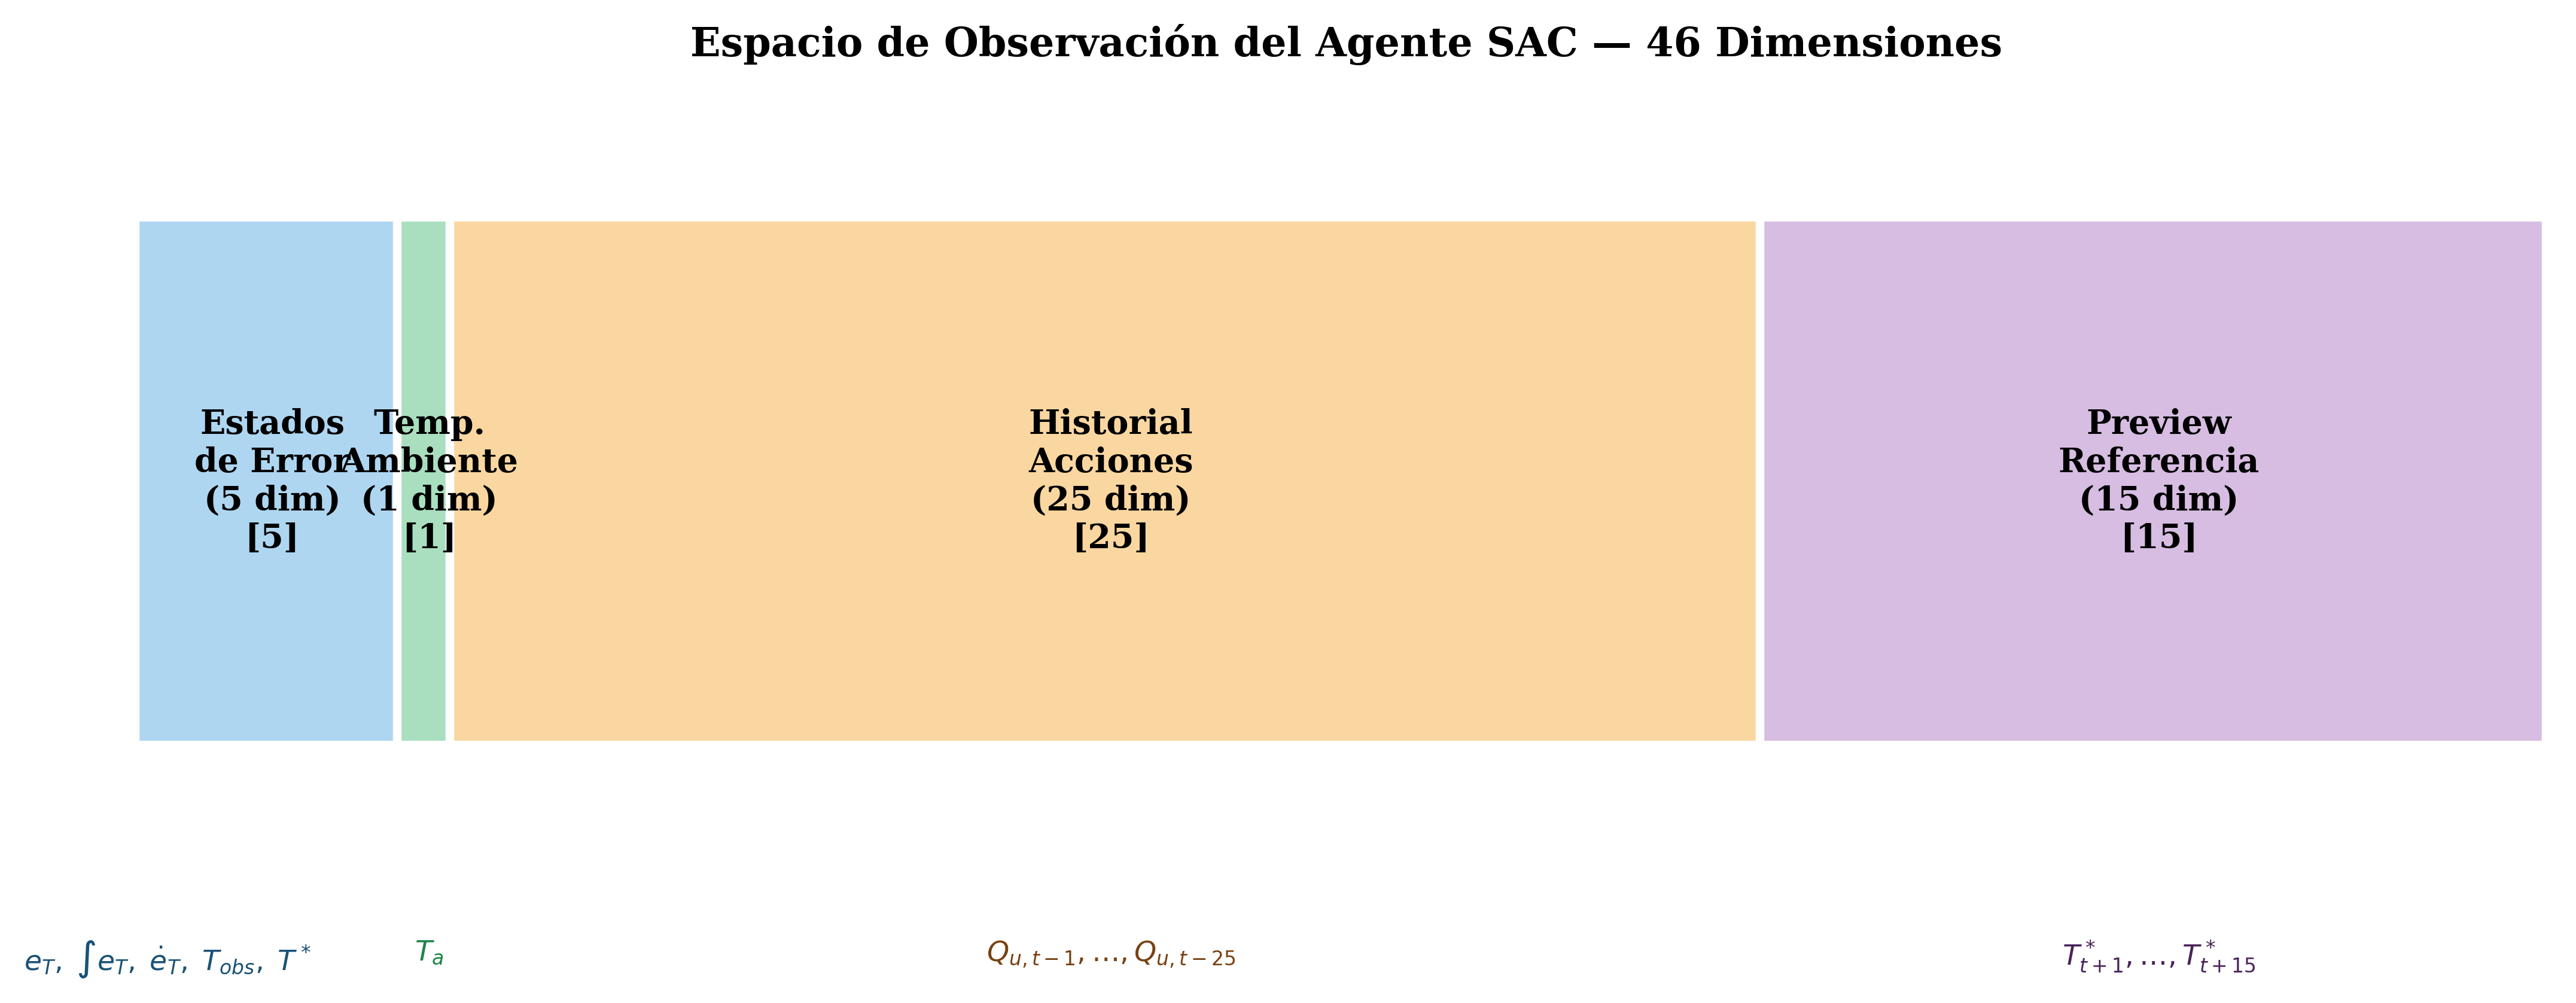
\includegraphics[width=\textwidth]{fig7_obs_space.png}
  \caption{Estructura del espacio de observación del agente SAC (46
           dimensiones): estados de error (azul), temperatura ambiente
           (verde), historial de 25 acciones (naranja) y previsualización
           de 15 pasos de la referencia (morado).}
  \label{fig:obs_space}
\end{figure}

La función de recompensa combina un término de seguimiento y energía con un
término de forma y una penalización asimétrica del sobreimpulso:

\begin{equation}
  \label{eq:reward_full}
  r_t = \underbrace{-(0.01\,\eT^2 + 10^{-4} \Qu^2)}_{r_{\mathrm{NMPC}}}
       \underbrace{-\, 0.3(|e_{T,\mathrm{obs}}| + 0.1\,|\Delta\Qu|)}_{r_{\mathrm{forma}}}
       \underbrace{-\, 0.02\,[\max(0,\, T - \Tref)]^2}_{r_{\mathrm{anti\text{-}OS}}}
\end{equation}

El término $r_{\mathrm{anti\text{-}OS}}$ penaliza asimétricamente el
sobreimpulso, reflejando procesos donde exceder el setpoint es más dañino
que no alcanzarlo. La arquitectura SAC se ilustra en la
Figura~\ref{fig:sac_arch}.

\begin{figure}[H]
  \centering
  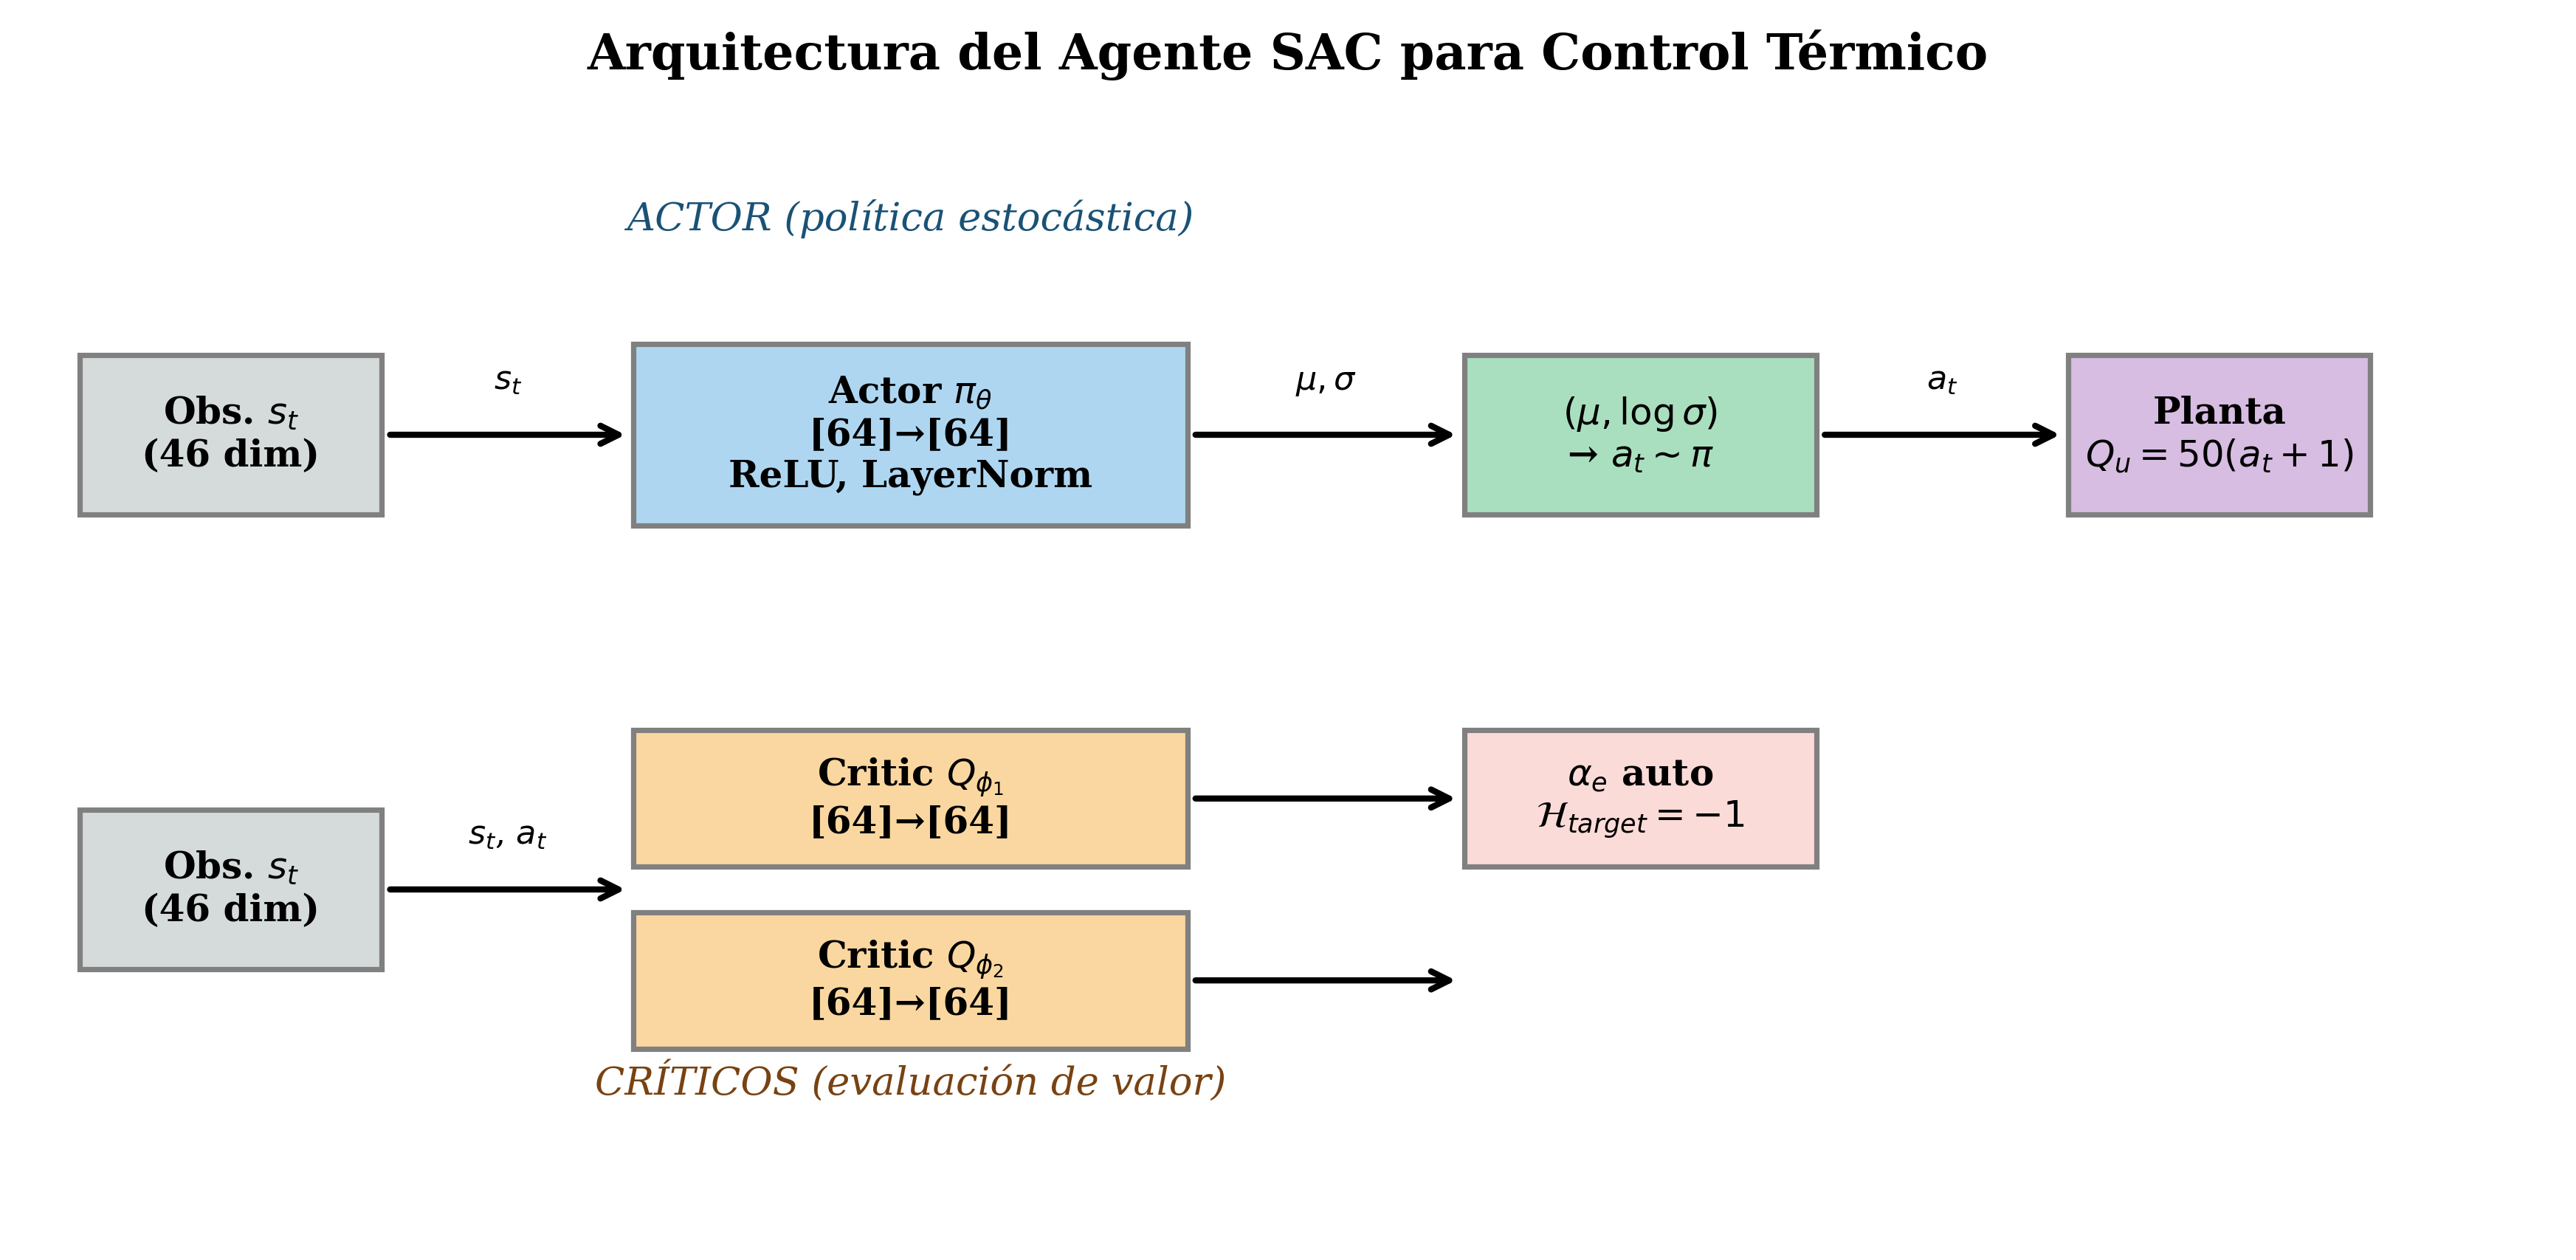
\includegraphics[width=0.92\textwidth]{fig8_sac_architecture.png}
  \caption{Arquitectura del agente SAC. El actor $\pi_\theta$ produce una
           distribución Gaussiana sobre $a_t \in [-1,1]$ que se mapea a
           $\Qu = 50(a_t+1)$. Dos críticos estiman el valor de acción y
           $\alpha_e$ se ajusta automáticamente.}
  \label{fig:sac_arch}
\end{figure}

\subsection{Arquitectura Residual NMPC-SAC}
\label{subsec:hybrid}

La arquitectura híbrida combina el NMPC con una corrección residual
aprendida por SAC:

\begin{equation}
  \label{eq:hybrid}
  Q_{u,k} = \operatorname{clip}\!\left(Q_{\mathrm{NMPC},k} + \Delta Q_k,\; 0,\; 100\right),
  \qquad \Delta Q_k \in [-15, +15]\,\%
\end{equation}

con red $[128,128]$ y un buffer pre-llenado con trayectorias del NMPC puro
($\Delta Q = 0$). Su observación es de 56 dimensiones y comparte la
estructura de la del SAC puro (Ec.~\eqref{eq:observation}) salvo en la
ventana de previsualización: cinco estados de error, la temperatura
ambiente, 25 acciones residuales pasadas y 25 pasos de previsualización de
la referencia ($5+1+25+25=56$). La previsualización se amplía de 15 a 25
pasos respecto al SAC puro, de modo que el NMPC-SAC dispone de \emph{más}
información anticipada que el SAC. Cualquier desventaja en su desempeño no
puede atribuirse, por tanto, a un déficit de información, sino a la
restricción de su espacio de acción.

Dos limitaciones estructurales explican por qué la corrección residual no
mejora --y puede empeorar-- al NMPC puro, y su manifestación cuantitativa se
documenta en la Sección~\ref{sec:results}.

La primera es la restricción del espacio de exploración. El solver SLSQP
converge a $Q_{\mathrm{NMPC}} \approx 25$--$35\,\%$ en estado
cuasi-estacionario, por la dominancia del término $R(U/100)^2$ cuando el
error es pequeño. Con $|\Delta Q| \leq 15\,\%$, el esfuerzo efectivo queda
confinado a $[10, 50]\,\%$, lo que impide alcanzar la región $\Qu > 70\,\%$
imprescindible en los escalones de gran amplitud desde arranque en frío.

La segunda es el efecto escalera de la base NMPC. A diferencia del NMPC puro,
que dispone del segundo completo de cómputo del PC para una sola optimización
(Sección~\ref{subsec:nmpc}), la arquitectura residual añade en cada paso la
inferencia de la política SAC y la fusión del residuo. Para mantener el lazo
combinado de optimización e inferencia dentro del presupuesto de tiempo real,
la base $Q_{\mathrm{NMPC}}$ se refresca cada $T_c = \SI{5}{\second}$ --se
cachea-- mientras el residuo SAC actúa a \SI{1}{\hertz}, lo que es admisible
porque la acción óptima del NMPC apenas varía entre pasos consecutivos. La
base cacheada produce una señal escalonada con saltos cada \SI{5}{\second}
($\approx \SI{0.2}{\hertz}$). Como la frecuencia de corte efectiva de la
planta es $f_c = 1/(2\pi\tau) \approx \SI{8.9e-4}{\hertz}$, esa excitación se
sitúa $\log_{10}(0.2/8.9\times10^{-4}) \approx 2.4$ décadas por encima del
ancho de banda del lazo. Combinada con el ruido del ADC, degrada la suavidad
del control y empeora el seguimiento, como confirman las métricas de la
Sección~\ref{subsec:dyn_stress}.

\subsection{Curriculum Learning: Protocolo de Cuatro Etapas}
\label{subsec:cl}

El protocolo (Figura~\ref{fig:curriculum}, Tabla~\ref{tab:curriculum})
expone al agente a complejidad creciente. El avance se dispara cuando la
recompensa media evaluada (política determinista, ventana $W=3$) supera el
umbral $\bar{r}_{\mathrm{th}}(s)$:

\begin{equation}
  \label{eq:cl_threshold}
  \frac{1}{W}\sum_{i=0}^{W-1} r_{\mathrm{eval},i} \geq \bar{r}_{\mathrm{th}}(s),
  \qquad W = 3
\end{equation}

Los umbrales $\{-166, -200, -340\}$ corresponden al $115\,\%$ de la
recompensa media del PI en esa etapa.

\begin{figure}[H]
  \centering
  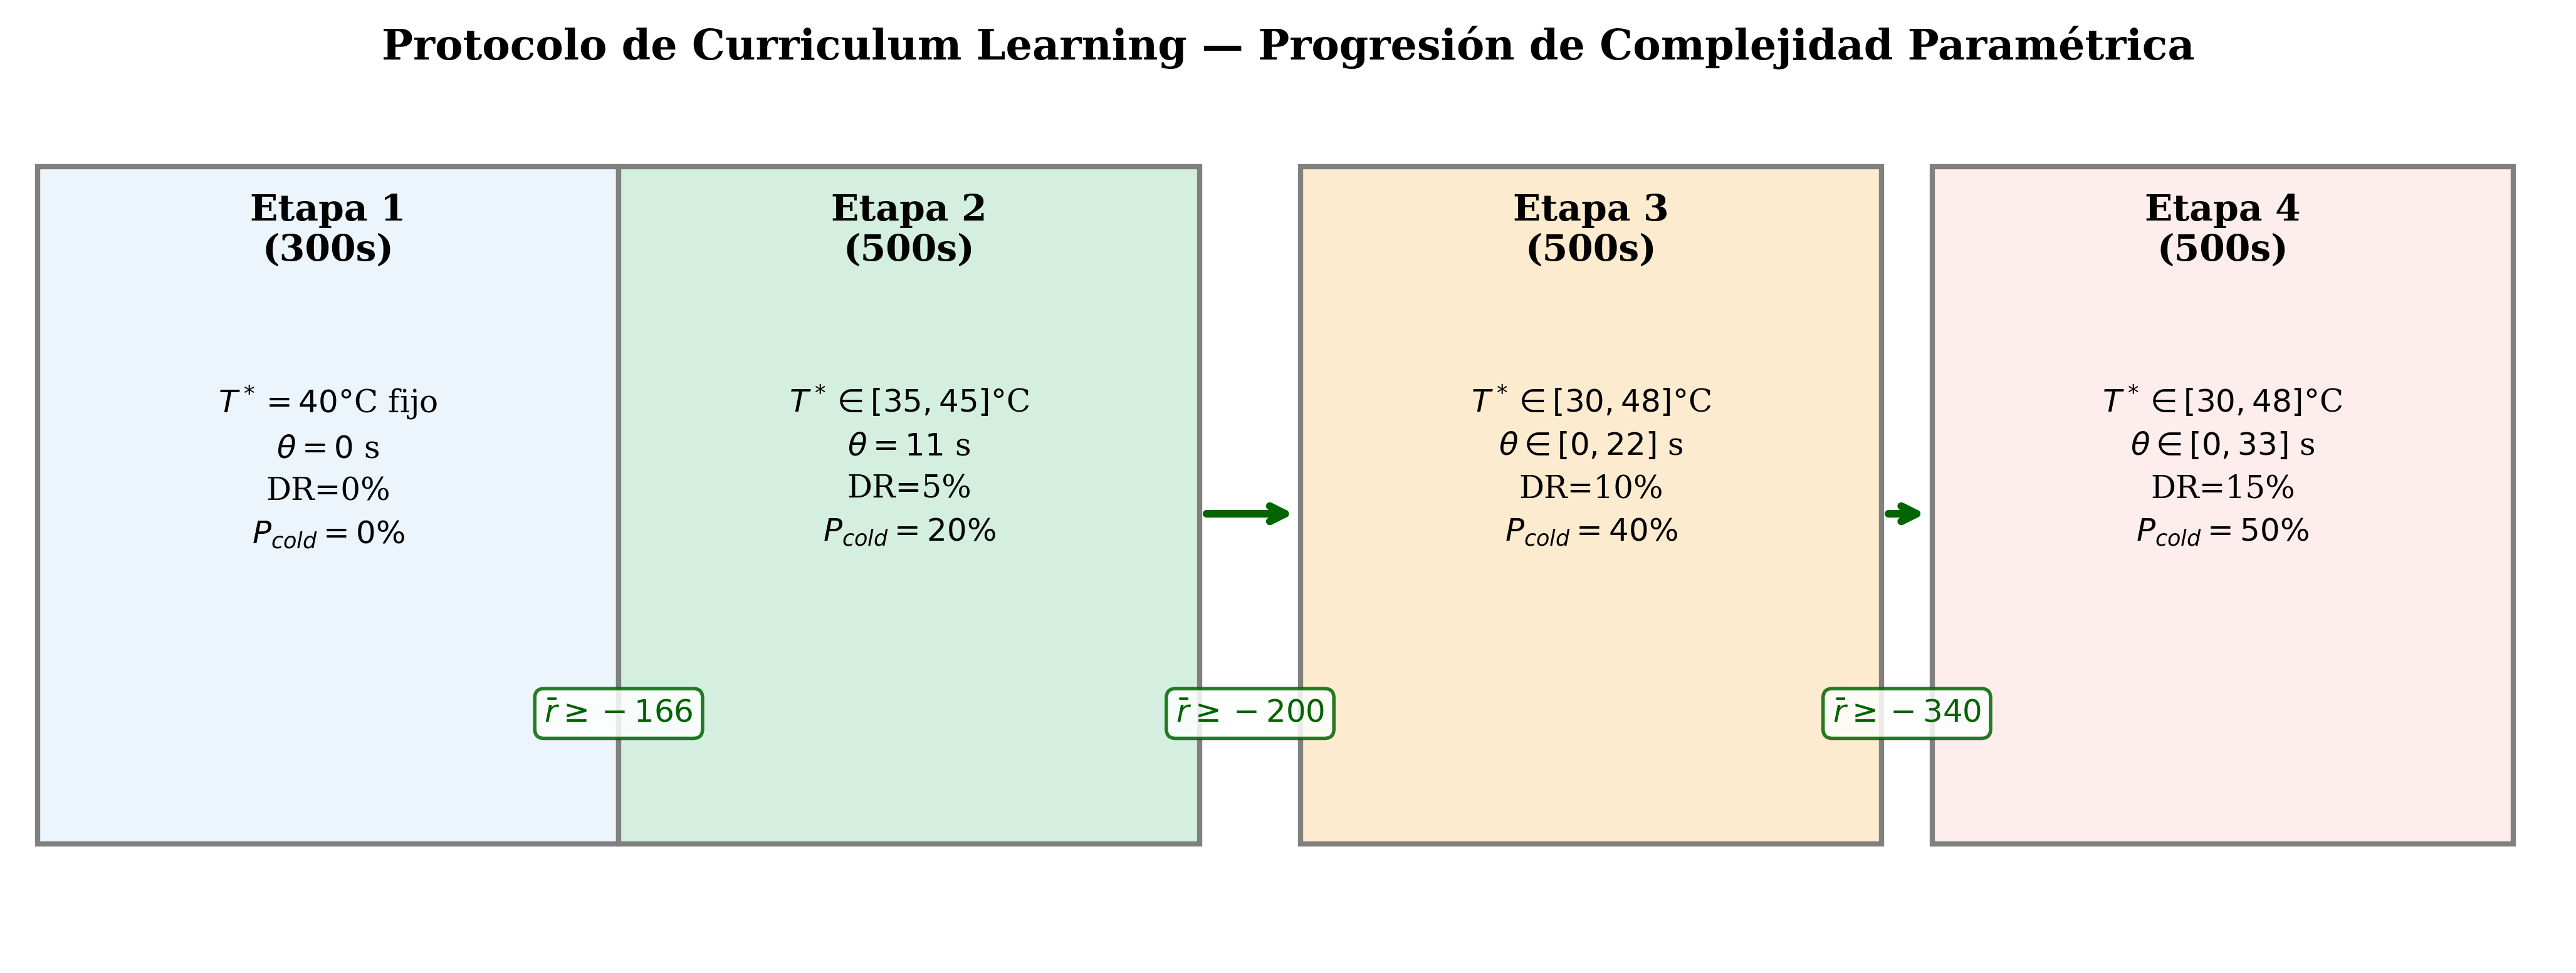
\includegraphics[width=\textwidth]{fig9_curriculum.png}
  \caption{Protocolo de Curriculum Learning. La complejidad crece
           progresivamente: $\theta_{\max}$ de 0 a \SI{33}{\second}, DR de
           0\,\% a $\pm 15\,\%$, $P_{\mathrm{cold}}$ de 0\,\% a 50\,\%.}
  \label{fig:curriculum}
\end{figure}

\begin{table}[H]
\caption{Configuración del Curriculum Learning. DR: Domain Randomization
         sobre $U_h$ y $K$. $P_{\mathrm{cold}}$: probabilidad de arranque
         en frío.}
\label{tab:curriculum}
\begin{tabular}{ccccccc}
\toprule
\textbf{Etapa} & $\Tref$ (\si{\celsius}) & $\theta$ (\si{\second}) &
\textbf{DR (\%)} & $T_{\mathrm{ep}}$ (\si{\second}) &
\textbf{Pert.\ $T_a$ (\si{\celsius})} & $P_{\mathrm{cold}}$ \\
\midrule
1 & 40 (fijo)  & 0          & 0  & 300 & 0       & 0\,\%  \\
2 & $[35, 45]$ & 11 (fijo)  & 5  & 500 & $\pm 1$ & 20\,\% \\
3 & $[30, 48]$ & $[0, 22]$  & 10 & 500 & $\pm 3$ & 40\,\% \\
4 & $[30, 48]$ & $[0, 33]$  & 15 & 500 & $\pm 5$ & 50\,\% \\
\bottomrule
\end{tabular}
\end{table}

\subsection{Hiperparámetros y Estudio de Ablación}
\label{subsec:ablation}

La Tabla~\ref{tab:hyperparams} lista los hiperparámetros (Stable-Baselines3
\cite{Raffin2021}). La planificación de entropía por etapa mantiene
$\alpha_e \in [\alpha_{\min}, \alpha_{\max}]$ (Tabla~\ref{tab:entropy}),
evitando el desbordamiento de $\alpha_e$ observado en versiones preliminares.

\begin{table}[H]
\caption{Hiperparámetros del agente SAC propuesto.}
\label{tab:hyperparams}
\begin{tabular}{llll}
\toprule
\textbf{Hiperparámetro} & \textbf{Valor} & \textbf{Hiperparámetro} & \textbf{Valor} \\
\midrule
Arquitectura de red & $[64, 64]$       & Tamaño de batch       & 256 \\
Tasa de aprendizaje & $3\times10^{-4}$ & $\tau$ (soft update)  & 0.005 \\
Tamaño del buffer   & 300{,}000        & $\gamma$ (descuento)  & 0.99 \\
Entropía objetivo   & $-1.0$           & \textit{ent\_coef}    & \texttt{auto} \\
Pre-llenado PI      & 300 episodios    & Pasos de aprendizaje  & 1 por paso \\
Timesteps totales   & 2{,}000{,}000    & N.\ entornos paralelos & 6 \\
\bottomrule
\end{tabular}
\end{table}

\begin{table}[H]
\begin{minipage}[t]{0.46\textwidth}
\caption{Planificación de la temperatura de entropía $\alpha_e$ por etapa.}
\label{tab:entropy}
\centering
\begin{tabular}{ccc}
\toprule
\textbf{Etapa} & $\alpha_{\min}$ & $\alpha_{\max}$ \\
\midrule
1 & 0.010 & 0.050 \\
2 & 0.005 & 0.025 \\
3 & 0.002 & 0.010 \\
4 & 0.001 & 0.005 \\
\bottomrule
\end{tabular}
\end{minipage}\hfill
\begin{minipage}[t]{0.50\textwidth}
\caption{Ablación de la red. Parámetros del actor para $[46\to n_1\to n_2\to 2]$.}
\label{tab:ablation}
\centering
\begin{tabular}{lcc}
\toprule
\textbf{Arquitectura} & \textbf{Parámetros} & \textbf{Problema} \\
\midrule
$[256,256]$ & $\sim\!78$k & Sobreajuste al ruido \\
$[128,128]$ & $\sim\!23$k & Exploración limitada \\
$[64,64]$\,(*) & $\sim\!7.1$k & Ninguno significativo \\
\bottomrule
\end{tabular}
\\[2pt]\footnotesize (*) Configuración propuesta.
\end{minipage}
\end{table}

El estudio de ablación (Tabla~\ref{tab:ablation}) muestra que la red
$[256,256]$ produjo sobreajuste al ruido residual del sensor (microajustes
en $\Qu$ para compensar fluctuaciones $< 0.1$\,°C que son ruido de ADC),
mientras que la red $[64,64]$ ($\sim\!7{,}100$ parámetros) alcanza el mejor
balance entre capacidad y robustez.

La Figura~\ref{fig:convergencia} muestra la curva de convergencia del
entrenamiento, medida por la recompensa media de episodio. La recompensa
asciende desde $\approx -2200$ y se estabiliza, y las líneas verticales marcan
las transiciones del Curriculum Learning. Dentro de cada etapa la política
converge a una meseta, y cada transición produce una caída transitoria porque
la tarea se endurece. La mayor parte del entrenamiento transcurre en la
Etapa~4, la más exigente (tiempo muerto hasta \SI{33}{\second}, Domain
Randomization de $\pm 15\,\%$ y arranques en frío), donde la recompensa se
estabiliza en torno a $-400$ durante cerca de $1.8\times10^{6}$ pasos sin
deriva, lo que evidencia la convergencia. Su menor valor absoluto respecto a
las etapas iniciales refleja la dificultad de la tarea, no una degradación de
la política.

\begin{figure}[H]
  \centering
  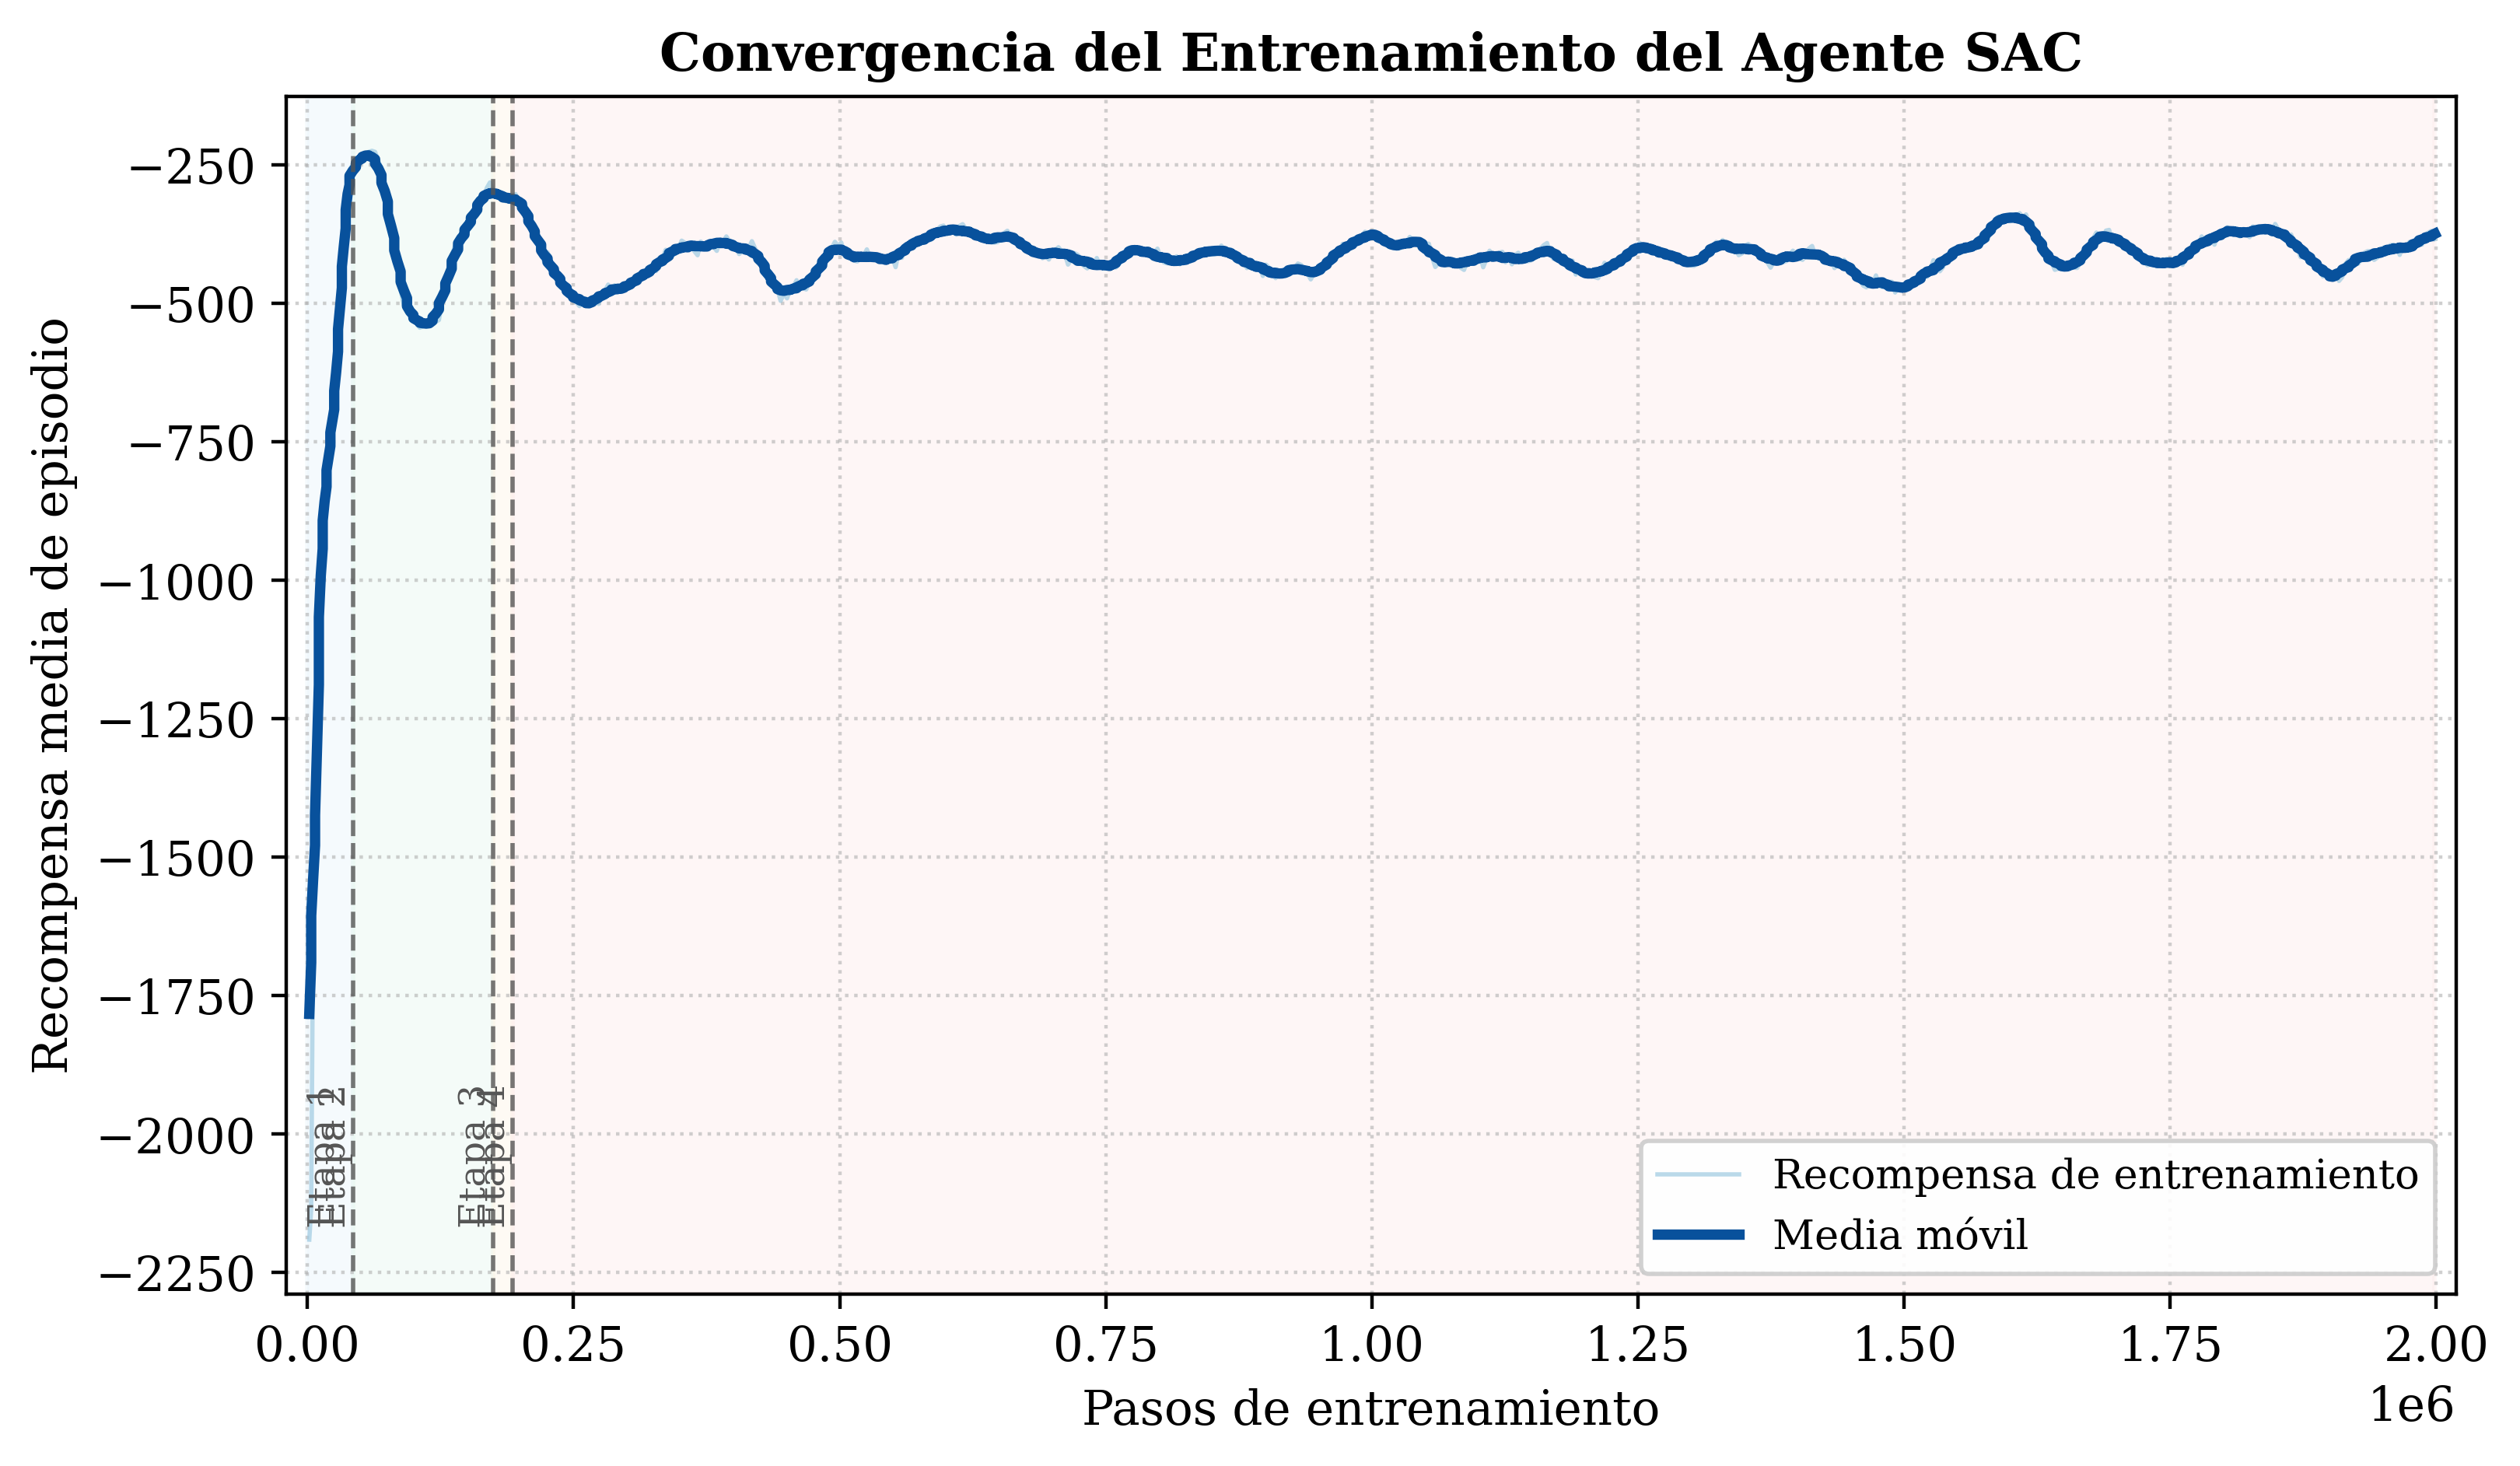
\includegraphics[width=0.9\textwidth]{fig11_convergencia.png}
  \caption{Convergencia del entrenamiento del agente SAC: recompensa media de
           episodio frente a los pasos de entrenamiento, con las transiciones
           del Curriculum Learning marcadas (líneas verticales) y el fondo
           coloreado por etapa. La política converge a una meseta dentro de
           cada etapa; la menor recompensa absoluta en la Etapa~4 corresponde
           a su mayor dificultad, no a una pérdida de desempeño.}
  \label{fig:convergencia}
\end{figure}

\subsection{Protocolo Experimental y Metodología Estadística}
\label{subsec:protocol}

Se diseñó un perfil de estrés dinámico de \SI{600}{\second} con cuatro
fases asimétricas:

\begin{equation}
  \label{eq:stress_profile}
  \Tref(t) =
  \begin{cases}
    \SI{35}{\celsius} & 0 \leq t < \SI{150}{\second} \\
    \SI{48}{\celsius} & \SI{150}{\second} \leq t < \SI{300}{\second} \\
    \SI{28}{\celsius} & \SI{300}{\second} \leq t < \SI{450}{\second} \\
    \SI{40}{\celsius} & \SI{450}{\second} \leq t \leq \SI{600}{\second}
  \end{cases}
\end{equation}

El perfil es adversarial por diseño. La Fase~1 parte de la temperatura
ambiente (arranque en frío) y la Fase~2 introduce un escalón de
$+\SI{13}{\celsius}$ que satura el actuador. En la Fase~3 el setpoint
$\Tref = \SI{28}{\celsius} < T_a$ es inalcanzable sin enfriamiento activo
($\Qu \geq 0$), lo que prueba el manejo de la restricción unilateral, y la
Fase~4 evalúa la recuperación.

Cada uno de los cuatro controladores se ejecutó en cuatro réplicas
independientes ($N=4$) sobre el mismo dispositivo TCLab, bajo condiciones
ambientales equivalentes ($T_a \approx \SI{32}{\celsius}$) y con al menos
\SI{5}{\minute} de enfriamiento entre corridas. El orden de las réplicas y de
los controladores se aleatorizó, en lugar de seguir una secuencia fija, de
modo que ningún controlador se evaluara de forma sistemática sobre un estado
térmico residual distinto y se preservara la independencia estadística entre
corridas. Se reporta la media $\pm$ desviación estándar de cada métrica y se
evalúa la significancia de la superioridad del SAC con el test no paramétrico
de Mann-Whitney~U, apropiado para muestras pequeñas sin supuesto de
normalidad.


% =====================================================================
\section{Resultados}
\label{sec:results}
% =====================================================================

\subsection{Evaluación en Simulación y Fidelidad Simulación-Hardware}
\label{subsec:sim_eval}

El agente SAC fue evaluado primero sobre el protocolo de tres pruebas del
artículo de referencia \cite{SozaMamani2025}, alcanzando un ISE de $40.85$ en
la Prueba~3 (la más exigente), consistente con el desempeño esperado en la Etapa~1 del
Curriculum y confirmando que el agente no regresiona en condiciones
moderadas. Como verificación adicional, los cuatro controladores se
simularon en el modelo ODE bajo el perfil de estrés con cuatro réplicas
(semillas distintas con ruido y DR). La Tabla~\ref{tab:metricas_sim}
muestra que el orden de desempeño en simulación
(SAC $<$ PI $<$ NMPC $<$ NMPC-SAC en ISE) es idéntico al observado en
hardware (Sección~\ref{subsec:dyn_stress}), validando la fidelidad del
simulador empleado en el entrenamiento.

\begin{table}[H]
\caption{Métricas en \emph{simulación} (modelo ODE, $N=4$ réplicas,
         media $\pm$ desv.\ est.). Corrobora el orden de desempeño del
         hardware.}
\label{tab:metricas_sim}
\begin{tabular}{lcccc}
\toprule
\textbf{Controlador} & \textbf{ISE} & \textbf{OS máx.\ (\si{\celsius})} &
\textbf{Energía (\%$\cdot$s)} & \textbf{TV} \\
\midrule
PI Clásico & $45{,}215 \pm 407$ & $19.6 \pm 0.1$ & $11{,}575 \pm 252$ & $508 \pm 15$ \\
NMPC puro  & $48{,}384 \pm 654$ & $21.8 \pm 0.1$ & $12{,}316 \pm 184$ & $259 \pm 4$ \\
NMPC-SAC   & $63{,}597 \pm 690$ & $24.0 \pm 0.2$ & $13{,}560 \pm 244$ & $301 \pm 12$ \\
SAC Puro   & $\mathbf{31{,}475 \pm 242}$ & $\mathbf{14.2 \pm 0.1}$ & $\mathbf{9{,}699 \pm 171}$ & $486 \pm 11$ \\
\bottomrule
\end{tabular}
\end{table}

\subsection{Sensibilidad del NMPC al Horizonte y a los Pesos}
\label{subsec:nmpc_sensitivity}

El NMPC de la Tabla~\ref{tab:metricas_sim} no supera al PI, y sus pesos se
heredaron de un protocolo distinto \cite{SozaMamani2025}, con un horizonte
$T_p = \SI{30}{\second}$ que equivale a apenas el $17\,\%$ de la constante de
tiempo ($T_p/\tau = 0.17$). Para descartar que se trate de un benchmark mal
sintonizado, se barrieron en simulación cuatro horizontes
($T_p \in \{30, 60, 90, 120\}$\,s) y cinco conjuntos de pesos sobre los dos
escenarios, con tres réplicas cada uno. Estas corridas son independientes de
las de la Tabla~\ref{tab:metricas_sim}, con las que coinciden dentro de la
desviación de muestreo. La Tabla~\ref{tab:nmpc_sens} reúne las configuraciones
más representativas.

\begin{table}[H]
\caption{Sensibilidad del NMPC en simulación (modelo ODE, $N=3$, media):
         efecto del horizonte $T_p$ y de los pesos sobre el ISE y el
         sobreimpulso máximo, en los escenarios de estrés y de setpoint
         constante. Conjuntos de pesos $(S,R,P_N)$: Referencia
         $=(0.0113,0.001,0.1513)$ \cite{SozaMamani2025}; $S$ alto
         $=(0.05,0.001,0.1513)$; $P_N$ alto $=(0.0113,0.001,0.5)$; Balance
         $=(0.05,0.0005,0.5)$. Mejor NMPC en \textbf{negrita}. El PI se
         incluye como referencia.}
\label{tab:nmpc_sens}
\setlength{\tabcolsep}{4pt}
\begin{tabular}{lccccc}
\toprule
\textbf{Pesos} & $T_p$ (\si{\second}) & \textbf{ISE estrés} &
\textbf{OS estrés (\si{\celsius})} & \textbf{ISE const.} &
\textbf{OS const.\ (\si{\celsius})} \\
\midrule
Referencia & 30  & $48{,}033$ & $21.8$ & $5{,}315$ & $6.25$ \\
Referencia & 60  & $59{,}554$ & $24.7$ & $4{,}671$ & $4.32$ \\
Referencia & 90  & $68{,}999$ & $26.6$ & $6{,}954$ & $7.82$ \\
$S$ alto   & 30  & $43{,}112$ & $20.3$ & $4{,}001$ & $6.03$ \\
$S$ alto   & 120 & $\mathbf{42{,}364}$ & $\mathbf{19.4}$ & $5{,}825$ & $6.40$ \\
$P_N$ alto & 60  & $65{,}874$ & $24.1$ & $4{,}541$ & $\mathbf{3.56}$ \\
Balance    & 30  & $43{,}170$ & $20.3$ & $\mathbf{3{,}936}$ & $6.00$ \\
\midrule
\emph{PI (referencia)} & --- & $44{,}844$ & $19.5$ & $2{,}866$ & $0.96$ \\
\bottomrule
\end{tabular}
\end{table}

Del barrido se desprenden tres conclusiones. Alargar el horizonte no mejora de
forma monótona: con los pesos de referencia, pasar de $T_p = 30$ a
\SI{90}{\second} \emph{empeora} el ISE de estrés de $48{,}033$ a $68{,}999$,
porque un horizonte largo sobre un modelo con incertidumbre paramétrica y un
solver de iteraciones limitadas acumula error de predicción. En el setpoint
constante aparece un óptimo intermedio cerca de $T_p = \SI{60}{\second}$, que
reduce el sobreimpulso de $\SI{6.25}{\celsius}$ a $\SI{3.56}{\celsius}$.
Aumentar el peso del error de etapa ($S = 0.05$) es la modificación más
efectiva, pues rebaja el ISE de estrés a $\approx 42{,}400$ y el de arranque a
$\approx 4{,}000$, lo que sitúa al NMPC al nivel del PI. La tercera, y la más
importante, es que ninguna de las veinte combinaciones evaluadas acerca el NMPC al
SAC. La mejor configuración alcanza un ISE de estrés de $42{,}364$, todavía un
$35\,\%$ por encima del SAC ($31{,}475$ en simulación), con un sobreimpulso de
$\SI{19.4}{\celsius}$ frente a los $\SI{14.2}{\celsius}$ del SAC.

Esto obliga a ser claro sobre el alcance del benchmark. Las
Tablas~\ref{tab:metricas_const} y~\ref{tab:metricas} reportan el NMPC con los
pesos de \cite{SozaMamani2025}, no el NMPC óptimo para este perfil. El presente
análisis acota cuánto podría mejorar con una resintonización específica y
muestra que ese margen no altera el orden de desempeño. La resintonización
completa en hardware, con $S = 0.05$ y un horizonte entre $60$ y
\SI{120}{\second}, queda señalada como verificación complementaria.

\subsection{Prueba de Setpoint Constante en Hardware}
\label{subsec:const_sp}

La Figura~\ref{fig:sp_const_4ctrl} muestra la respuesta de los cuatro
controladores a un setpoint constante de $\Tref \approx \SI{40.8}{\celsius}$
desde arranque en frío, y la Tabla~\ref{tab:metricas_const} resume sus
métricas. En esta condición estacionaria el PI es el más preciso (menor ISE,
IAE e ITAE), resultado esperado dado que fue diseñado analíticamente para
regulación en torno a un punto fijo. El SAC lo sigue de cerca (ISE
$+23.9\,\%$ sobre el PI). Los esquemas basados en NMPC presentan mayor error
y sobreimpulso en el transitorio de arranque. El NMPC puro sobrepasa
$\SI{6.3}{\celsius}$ y el NMPC-SAC $\SI{3.6}{\celsius}$, frente a menos de
\SI{1}{\celsius} de PI y SAC. Como muestra el análisis de sensibilidad
(Sección~\ref{subsec:nmpc_sensitivity}), una resintonización del NMPC reduce
este sobreimpulso en simulación, pero no lo lleva al nivel del PI. El SAC exhibe la mayor Variación Total,
reflejo del chattering de su política estocástica
(Sección~\ref{subsec:disc_chattering}). Este escenario, en el que el SAC
no domina, contrasta con la prueba de estrés (Sección~\ref{subsec:dyn_stress})
y delimita el régimen donde el aporte del agente es decisivo: las
transiciones severas, no la regulación estacionaria.

\begin{figure}[H]
  \centering
  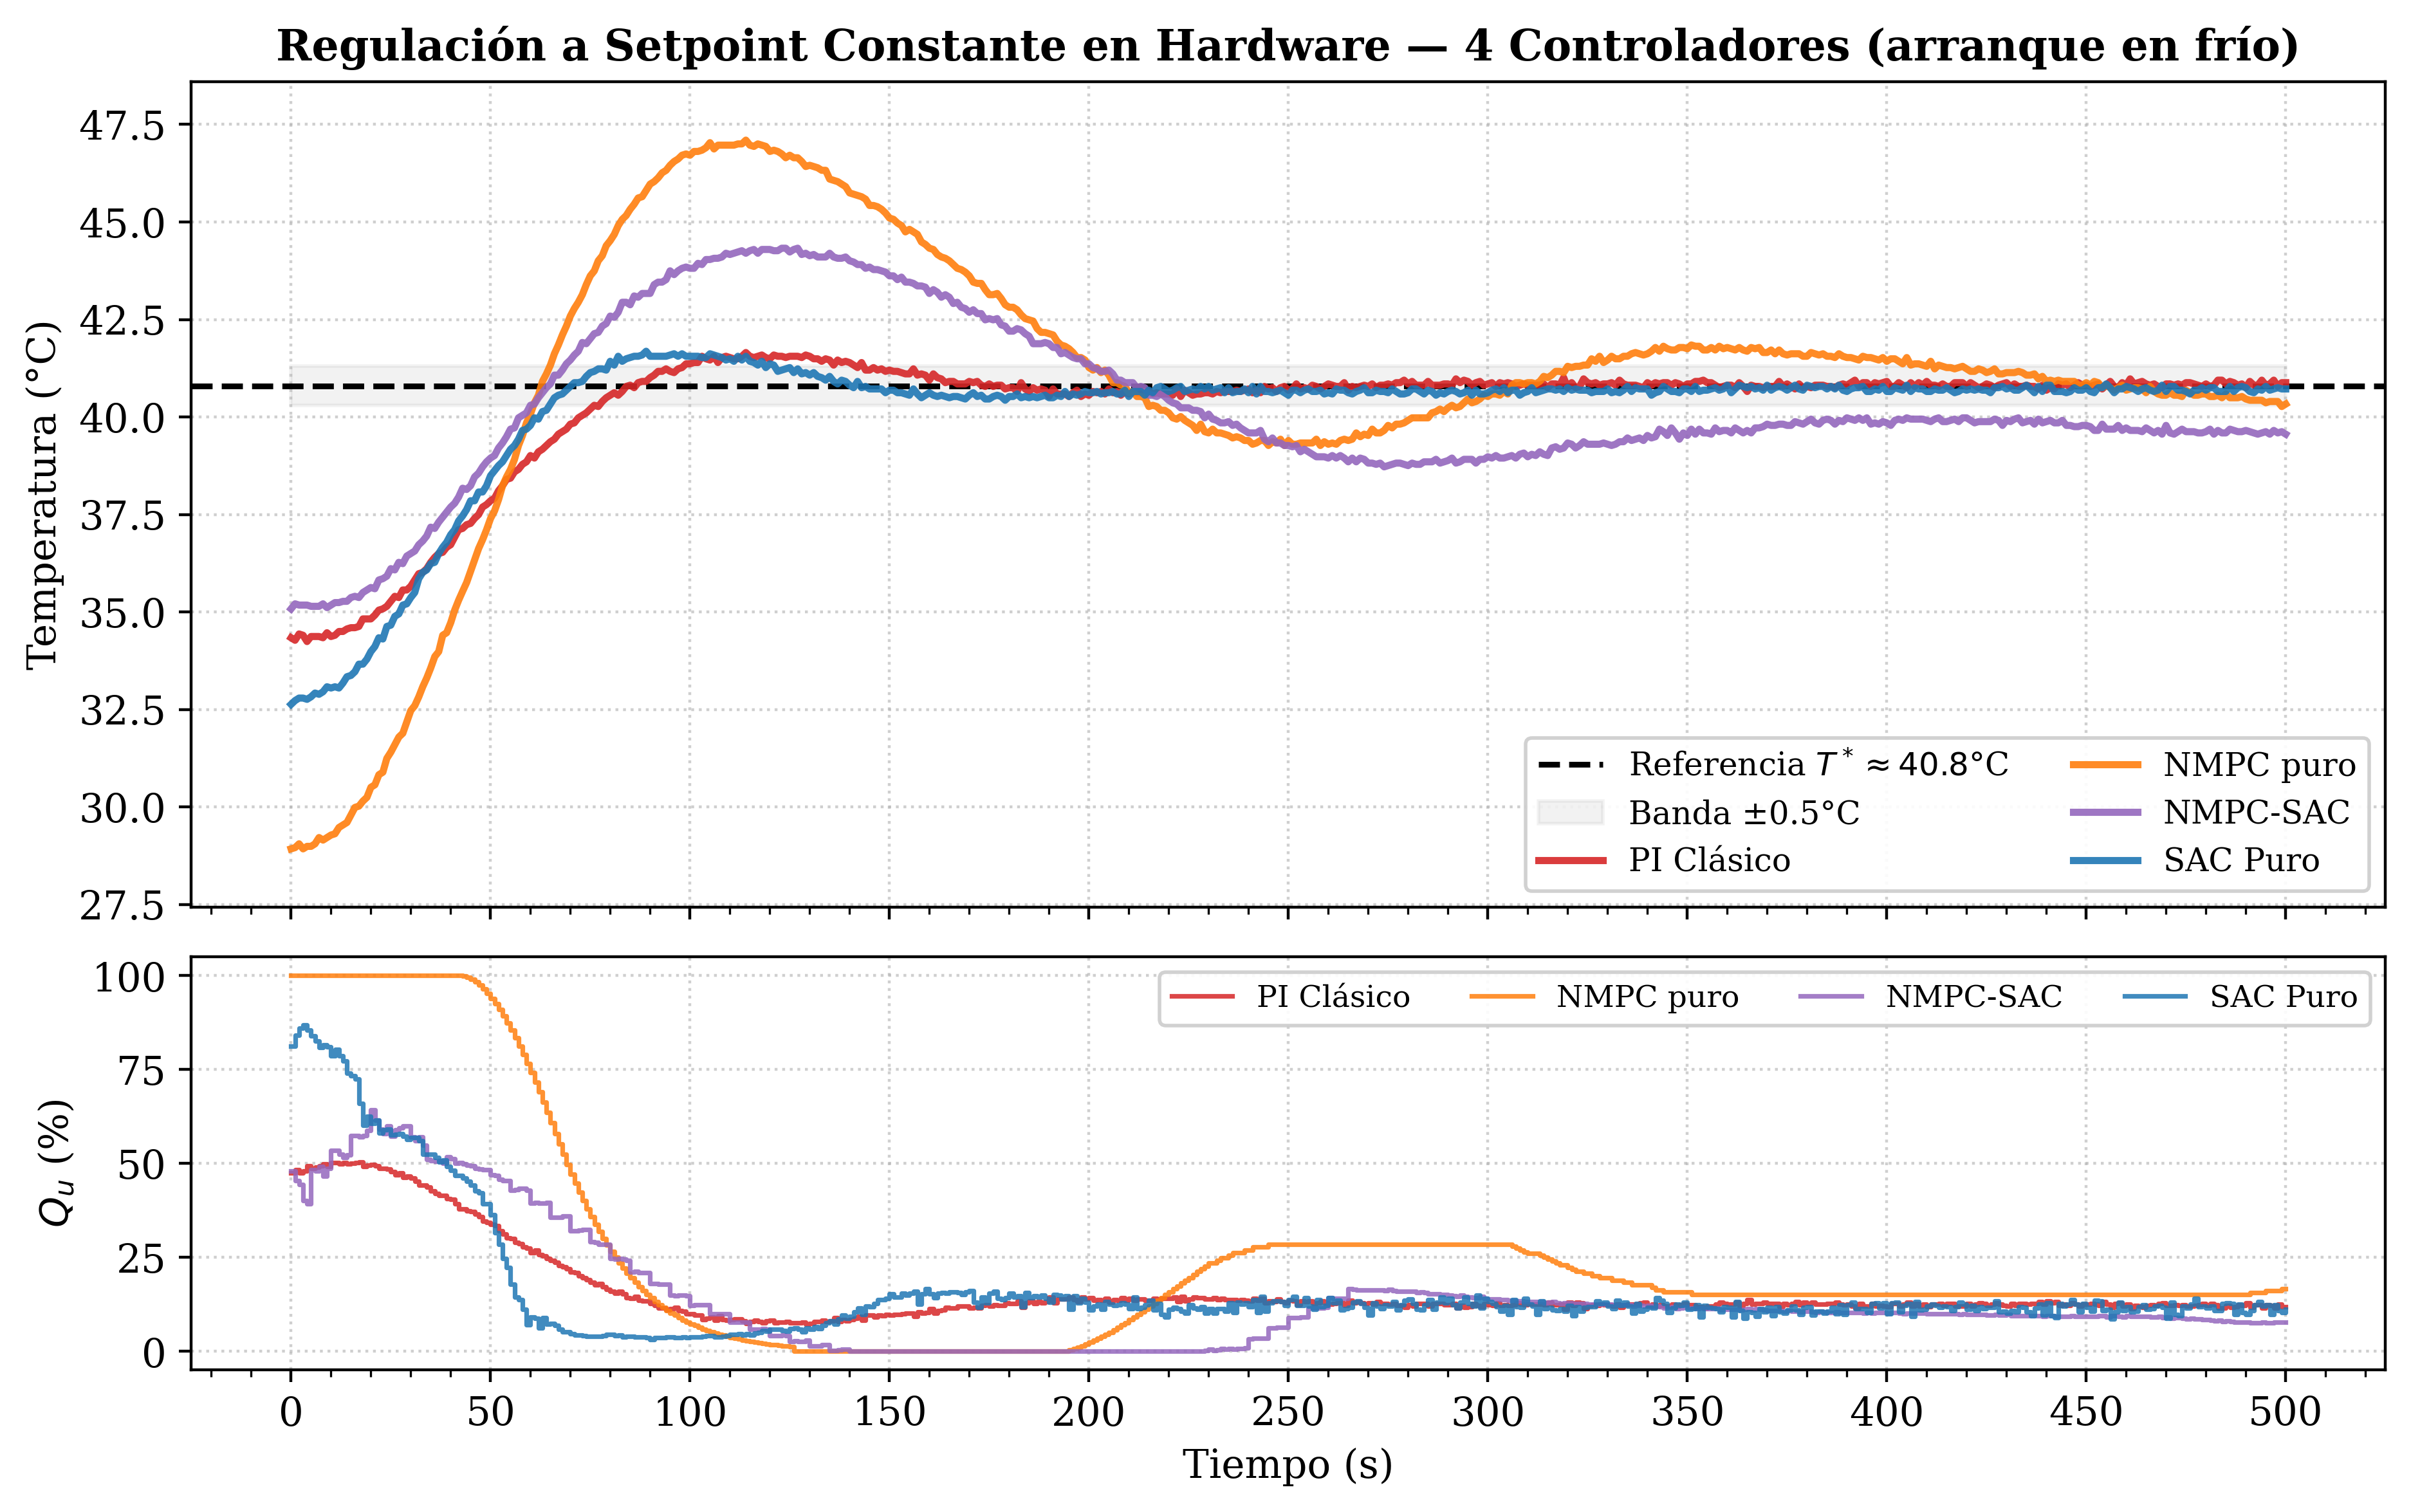
\includegraphics[width=\textwidth]{fig_sp_const_4ctrl.png}
  \caption{Regulación a setpoint constante en hardware
           ($\Tref \approx \SI{40.8}{\celsius}$, arranque en frío) para los
           cuatro controladores. Panel superior: temperatura medida y banda
           de tolerancia $\pm\SI{0.5}{\celsius}$. Panel inferior: esfuerzo de
           control $\Qu(t)$. PI y SAC convergen sin sobreimpulso apreciable;
           NMPC y NMPC-SAC sobrepasan durante el transitorio.}
  \label{fig:sp_const_4ctrl}
\end{figure}

\begin{table}[H]
\caption{Métricas en setpoint constante en hardware
         ($\Tref \approx \SI{40.8}{\celsius}$, arranque en frío). Valores
         óptimos en \textbf{negrita}.}
\label{tab:metricas_const}
\begin{tabular}{lcccccc}
\toprule
\textbf{Controlador} & \textbf{ISE} & \textbf{IAE} & \textbf{ITAE} &
\textbf{OS (\si{\celsius})} & \textbf{Energía (\%$\cdot$s)} & \textbf{TV} \\
\midrule
PI Clásico & \textbf{1{,}568.5} & \textbf{375.9} & \textbf{20{,}813}
           & \textbf{0.85} & 8{,}068 & 231.6 \\
NMPC puro  & 7{,}103.1 & 1{,}200.5 & 138{,}931 & 6.30 & 12{,}903 & \textbf{143.4} \\
NMPC-SAC   & 2{,}416.0 & 905.8 & 168{,}976 & 3.55 & \textbf{7{,}216} & 175.9 \\
SAC Puro   & 1{,}943.1 & 392.4 & 22{,}128 & 0.91 & 8{,}085 & 613.6 \\
\bottomrule
\end{tabular}
\end{table}

\subsection{Prueba de Estrés Dinámico: Comparación de los Cuatro Controladores}
\label{subsec:dyn_stress}

La Tabla~\ref{tab:metricas} presenta las métricas de los cuatro
controladores en hardware (media $\pm$ desviación estándar sobre $N=4$
réplicas). La Figura~\ref{fig:barras} las visualiza con barras de error, y
la Figura~\ref{fig:stress_main} muestra la respuesta temporal de la réplica
representativa (mediana de ISE) de cada controlador.

\begin{table}[H]
\caption{Métricas de la prueba de estrés dinámico en hardware real
         ($N=4$ réplicas, media $\pm$ desviación estándar). Valores óptimos
         en \textbf{negrita}. Última fila: mejora relativa del SAC respecto
         al mejor de los otros tres controladores en cada métrica.}
\label{tab:metricas}
\setlength{\tabcolsep}{4pt}
\begin{tabular}{lcccccc}
\toprule
\textbf{Controlador} & \textbf{ISE} & \textbf{IAE} & \textbf{ITAE} &
\textbf{OS máx.\ (\si{\celsius})} & \textbf{Energía (\%$\cdot$s)} & \textbf{TV} \\
\midrule
PI Clásico & $44{,}650 \pm 271$ & $3{,}493 \pm 49$ & $1{,}100{,}268 \pm 4361$
           & $20.5 \pm 0.1$ & $14{,}300 \pm 475$ & $392 \pm 5$ \\
NMPC puro  & $44{,}557 \pm 513$ & $3{,}768 \pm 49$ & $1{,}149{,}326 \pm 2751$
           & $22.2 \pm 0.0$ & $15{,}551 \pm 161$ & $369 \pm 14$ \\
NMPC-SAC   & $55{,}493 \pm 1545$ & $4{,}001 \pm 71$ & $1{,}224{,}277 \pm 29{,}273$
           & $22.9 \pm 0.2$ & $15{,}372 \pm 31$ & $\mathbf{302 \pm 13}$ \\
SAC Puro   & $\mathbf{30{,}137 \pm 301}$ & $\mathbf{3{,}486 \pm 20}$
           & $\mathbf{982{,}262 \pm 3722}$ & $\mathbf{14.0 \pm 0.1}$
           & $\mathbf{13{,}746 \pm 260}$ & $725 \pm 23$ \\
\midrule
\textit{Mejora SAC} & $-32.4\,\%$ & $-0.2\,\%$ & $-10.7\,\%$ & $-31.8\,\%$
                    & $-3.9\,\%$ & $+140\,\%$ \\
\bottomrule
\end{tabular}
\end{table}

\begin{figure}[H]
  \centering
  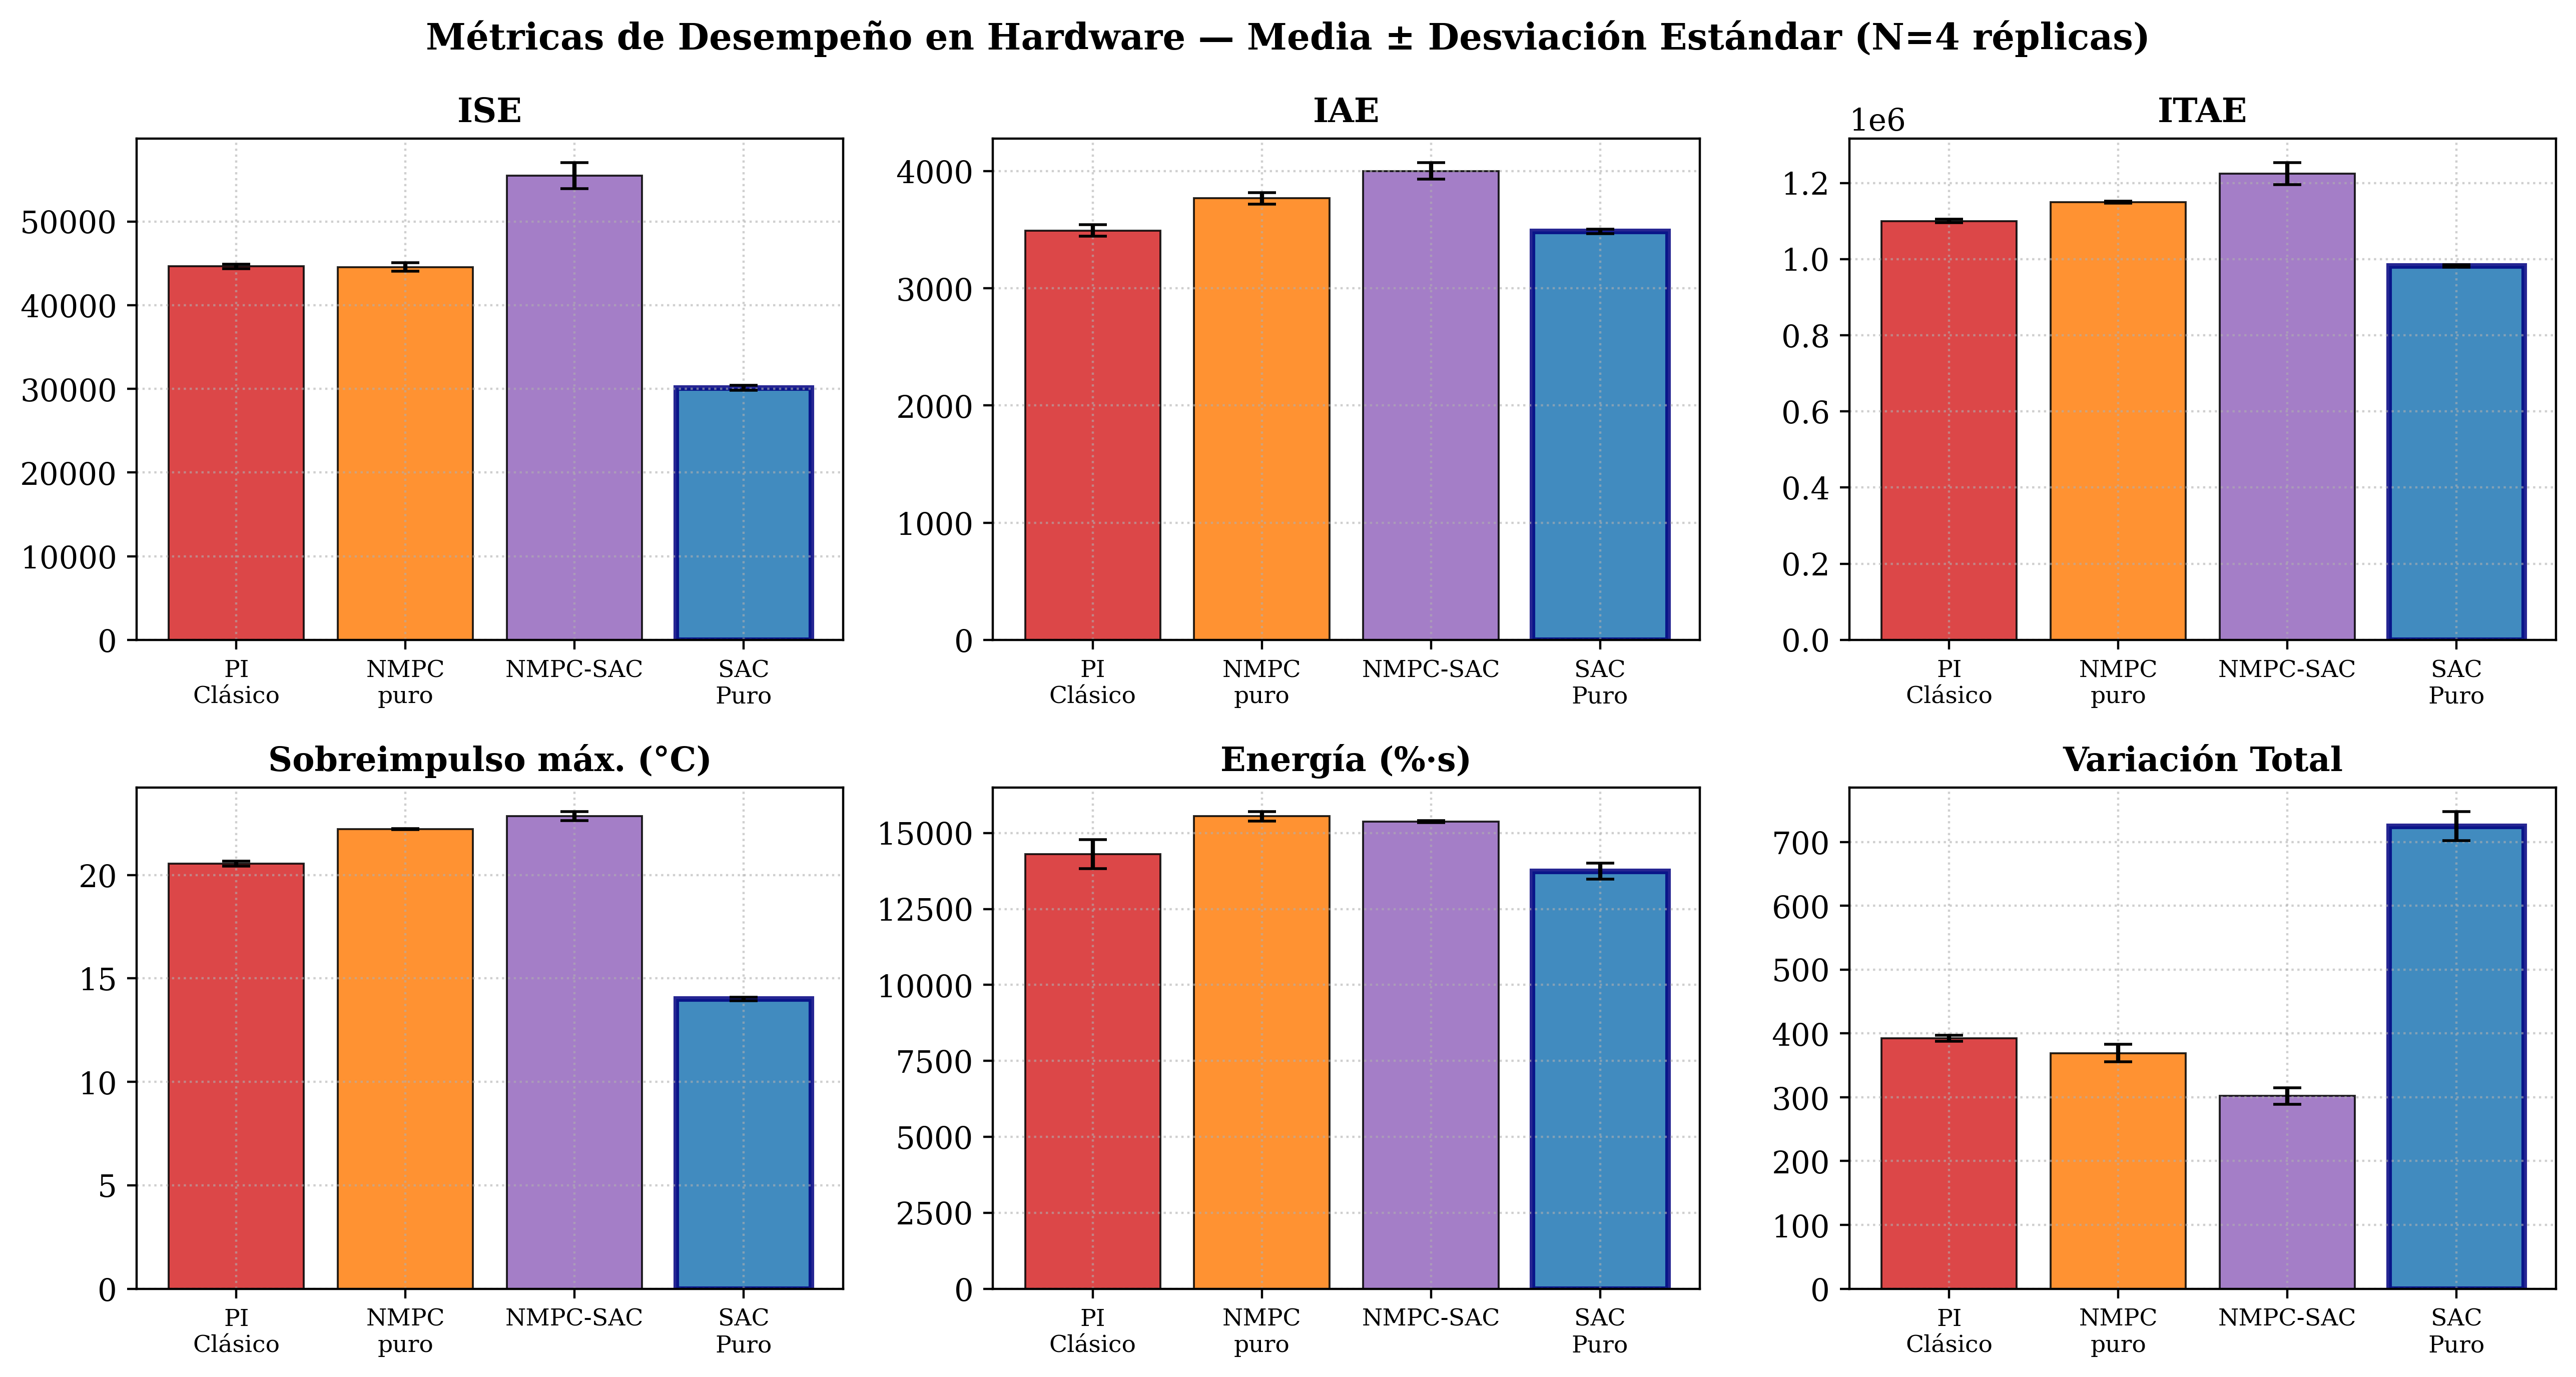
\includegraphics[width=\textwidth]{fig10_barras_estadisticas.png}
  \caption{Métricas de desempeño en hardware (media $\pm$ desviación
           estándar, $N=4$ réplicas) para los cuatro controladores. El SAC
           (barra resaltada) domina en ISE, IAE, ITAE, sobreimpulso y
           energía, y presenta la mayor Variación Total (chattering).}
  \label{fig:barras}
\end{figure}

\begin{figure}[H]
  \centering
  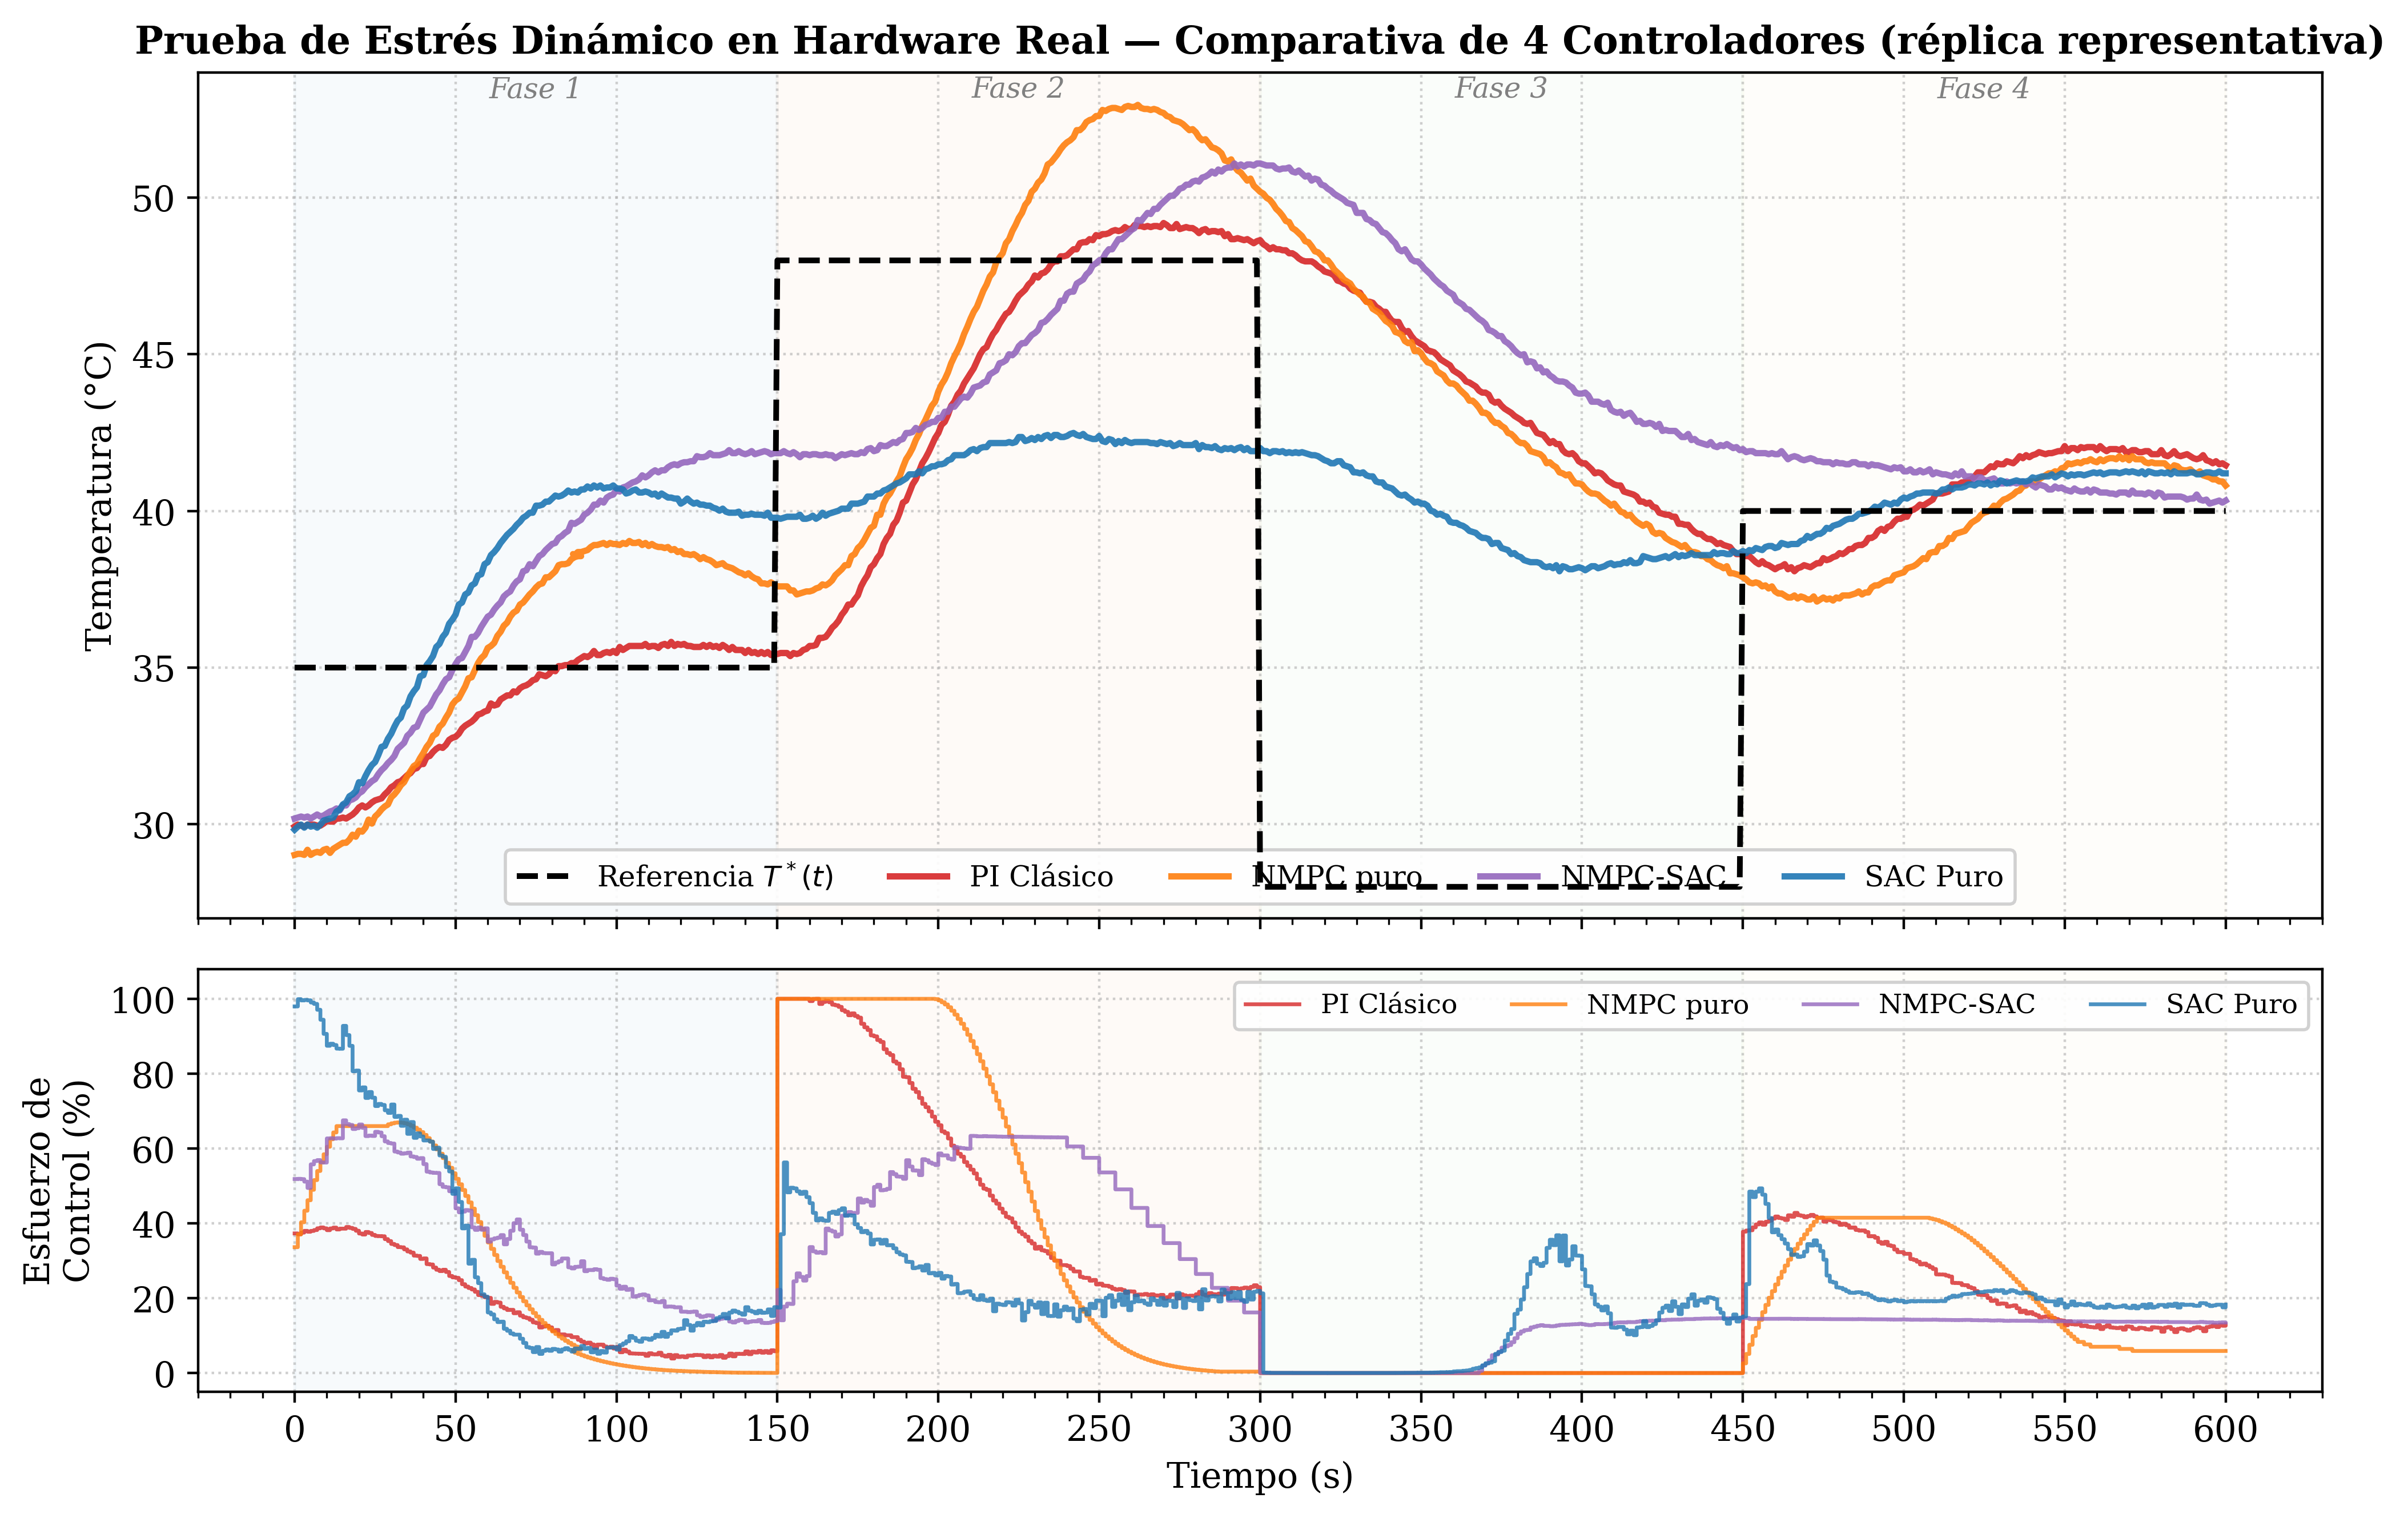
\includegraphics[width=\textwidth]{fig1_comparativa_principal.png}
  \caption{\textbf{Gráfica principal:} prueba de estrés dinámico en
           hardware real, réplica representativa de cada controlador. Panel
           superior: temperatura y referencia $\Tref(t)$. Panel inferior:
           señal de control $\Qu(t)$. Las bandas de color indican las
           cuatro fases del perfil.}
  \label{fig:stress_main}
\end{figure}

El SAC domina en cinco de las seis métricas. En ISE supera al PI en
$32.5\,\%$, al NMPC en $32.4\,\%$ y al NMPC-SAC en $45.7\,\%$. En IAE, el
SAC ($3{,}486$) es estadísticamente equivalente al PI ($3{,}493$, diferencia
$-0.2\,\%$) y claramente superior al NMPC ($-7.5\,\%$) y al NMPC-SAC
($-12.9\,\%$). Su única desventaja es la Variación Total, donde es el peor
($725$ frente a $302$--$392$): el costo de su política estocástica de alta
frecuencia y baja amplitud, analizado en la
Sección~\ref{subsec:disc_chattering}. El NMPC-SAC resultó el peor en ISE,
IAE, ITAE, sobreimpulso y energía, confirmando cuantitativamente el
diagnóstico de la Sección~\ref{subsec:hybrid}: su corrección residual
acotada y el efecto escalera del solver le impiden mejorar sobre el NMPC
puro, e incluso lo degradan.

\subsection{Análisis de Significancia Estadística}
\label{subsec:stats}

El test de Mann-Whitney U (alternativa unilateral SAC $<$ comparador,
métrica ISE) arroja $U = 0$ y $p = 0.0143$ para las tres comparaciones
(SAC vs.\ PI, SAC vs.\ NMPC, SAC vs.\ NMPC-SAC). El valor $p = 0.0143$ es el
mínimo alcanzable con $N=4$ por grupo y corresponde a la separación completa
de las distribuciones: todas las réplicas del SAC presentan un ISE inferior
al de todas las réplicas de cada comparador. La superioridad del SAC en ISE
es por tanto estadísticamente significativa al nivel $\alpha = 0.05$.

\subsection{Análisis Fase a Fase}
\label{subsec:phase_analysis}

La Tabla~\ref{tab:phase_stats} desglosa el comportamiento por fase de la
réplica representativa. En la Fase~2 (escalón de calentamiento), el SAC es
el único controlador sin sobreimpulso ($\SI{0.0}{\celsius}$ sobre el
setpoint), porque su $\Qu$ máximo es $56.3\,\%$ --nunca satura-- frente al
$100\,\%$ del PI y del NMPC. En la Fase~3 (enfriamiento pasivo), todos los
controladores son incapaces de alcanzar $\Tref = \SI{28}{\celsius} < T_a$,
pero el SAC entra a esta fase a $\SI{42.0}{\celsius}$ mientras PI, NMPC y
NMPC-SAC lo hacen a $48.7$, $50.2$ y $\SI{51.1}{\celsius}$ respectivamente,
lo que reduce su sobreimpulso de fase a $\SI{14.0}{\celsius}$ frente a
$20.7$--$\SI{23.1}{\celsius}$. La Fase~1 evidencia la única debilidad del
SAC: un sobreimpulso de arranque de $\SI{5.8}{\celsius}$
(Sección~\ref{subsec:disc_causal}).

\begin{table}[H]
\caption{Estadísticas por fase (réplica representativa). OS: sobreimpulso
         sobre el setpoint de la fase; MaxQu/MinQu: extremos del esfuerzo
         de control.}
\label{tab:phase_stats}
\setlength{\tabcolsep}{4.5pt}
\begin{tabular}{llccccc}
\toprule
\textbf{Fase} & \textbf{Controlador} &
\textbf{MaxT (°C)} & \textbf{MinT (°C)} & \textbf{OS (°C)} &
\textbf{MaxQu (\%)} & \textbf{MinQu (\%)} \\
\midrule
\multirow{4}{*}{1 (35°C)}
  & PI Clásico & 35.82 & 29.92 & \textbf{0.82} & 39.0 & 3.9 \\
  & NMPC puro  & 39.04 & 29.02 & 4.04 & 67.0 & 0.0 \\
  & NMPC-SAC   & 41.94 & 30.18 & 6.94 & 67.5 & 13.4 \\
  & SAC Puro   & 40.81 & 29.82 & 5.81 & 99.9 & 5.1 \\
\midrule
\multirow{4}{*}{2 (48°C)}
  & PI Clásico & 49.19 & 35.37 & 1.19 & 100.0 & 19.9 \\
  & NMPC puro  & 52.96 & 37.33 & 4.96 & 100.0 & 0.4 \\
  & NMPC-SAC   & 51.09 & 41.69 & 3.09 & 63.4 & 14.1 \\
  & SAC Puro   & 42.49 & 39.75 & \textbf{0.00} & 56.3 & 13.8 \\
\midrule
\multirow{4}{*}{3 (28°C)}
  & PI Clásico & 48.65 & 38.62 & 20.65 & 0.0 & 0.0 \\
  & NMPC puro  & 50.19 & 37.95 & 22.19 & 0.0 & 0.0 \\
  & NMPC-SAC   & 51.09 & 41.94 & 23.09 & 14.7 & 0.0 \\
  & SAC Puro   & 42.01 & 38.08 & \textbf{14.01} & 36.8 & 0.0 \\
\midrule
\multirow{4}{*}{4 (40°C)}
  & PI Clásico & 42.07 & 38.08 & 2.07 & 42.8 & 10.9 \\
  & NMPC puro  & 41.75 & 37.11 & 1.75 & 41.5 & 2.6 \\
  & NMPC-SAC   & 41.98 & 40.23 & 1.98 & 14.7 & 13.5 \\
  & SAC Puro   & 41.27 & 38.66 & \textbf{1.27} & 49.3 & 15.1 \\
\bottomrule
\end{tabular}
\end{table}

\subsection{Trayectoria del Error, Windup, Enfriamiento e Integrales}

El error de seguimiento $e(t) = \Tref(t) - T(t)$ de los cuatro controladores
se muestra en la Figura~\ref{fig:error}. En el escalón de calentamiento de la
Fase~2 (Figura~\ref{fig:zoom_windup}), el SAC reduce $\Qu$ con antelación y no
sobrepasa, mientras el PI y el NMPC saturan. Durante el enfriamiento pasivo de
la Fase~3 (Figura~\ref{fig:zoom_cooling}), ningún controlador logra bajar de la
temperatura ambiente $T_a$, marcada como límite físico. Las integrales
acumuladas de energía e ISE (Figura~\ref{fig:integrals}) concentran la
divergencia del ISE en la Fase~3, donde la mayor temperatura de entrada del PI,
el NMPC y el NMPC-SAC penaliza el error cuadrático.

\begin{figure}[H]
  \centering
  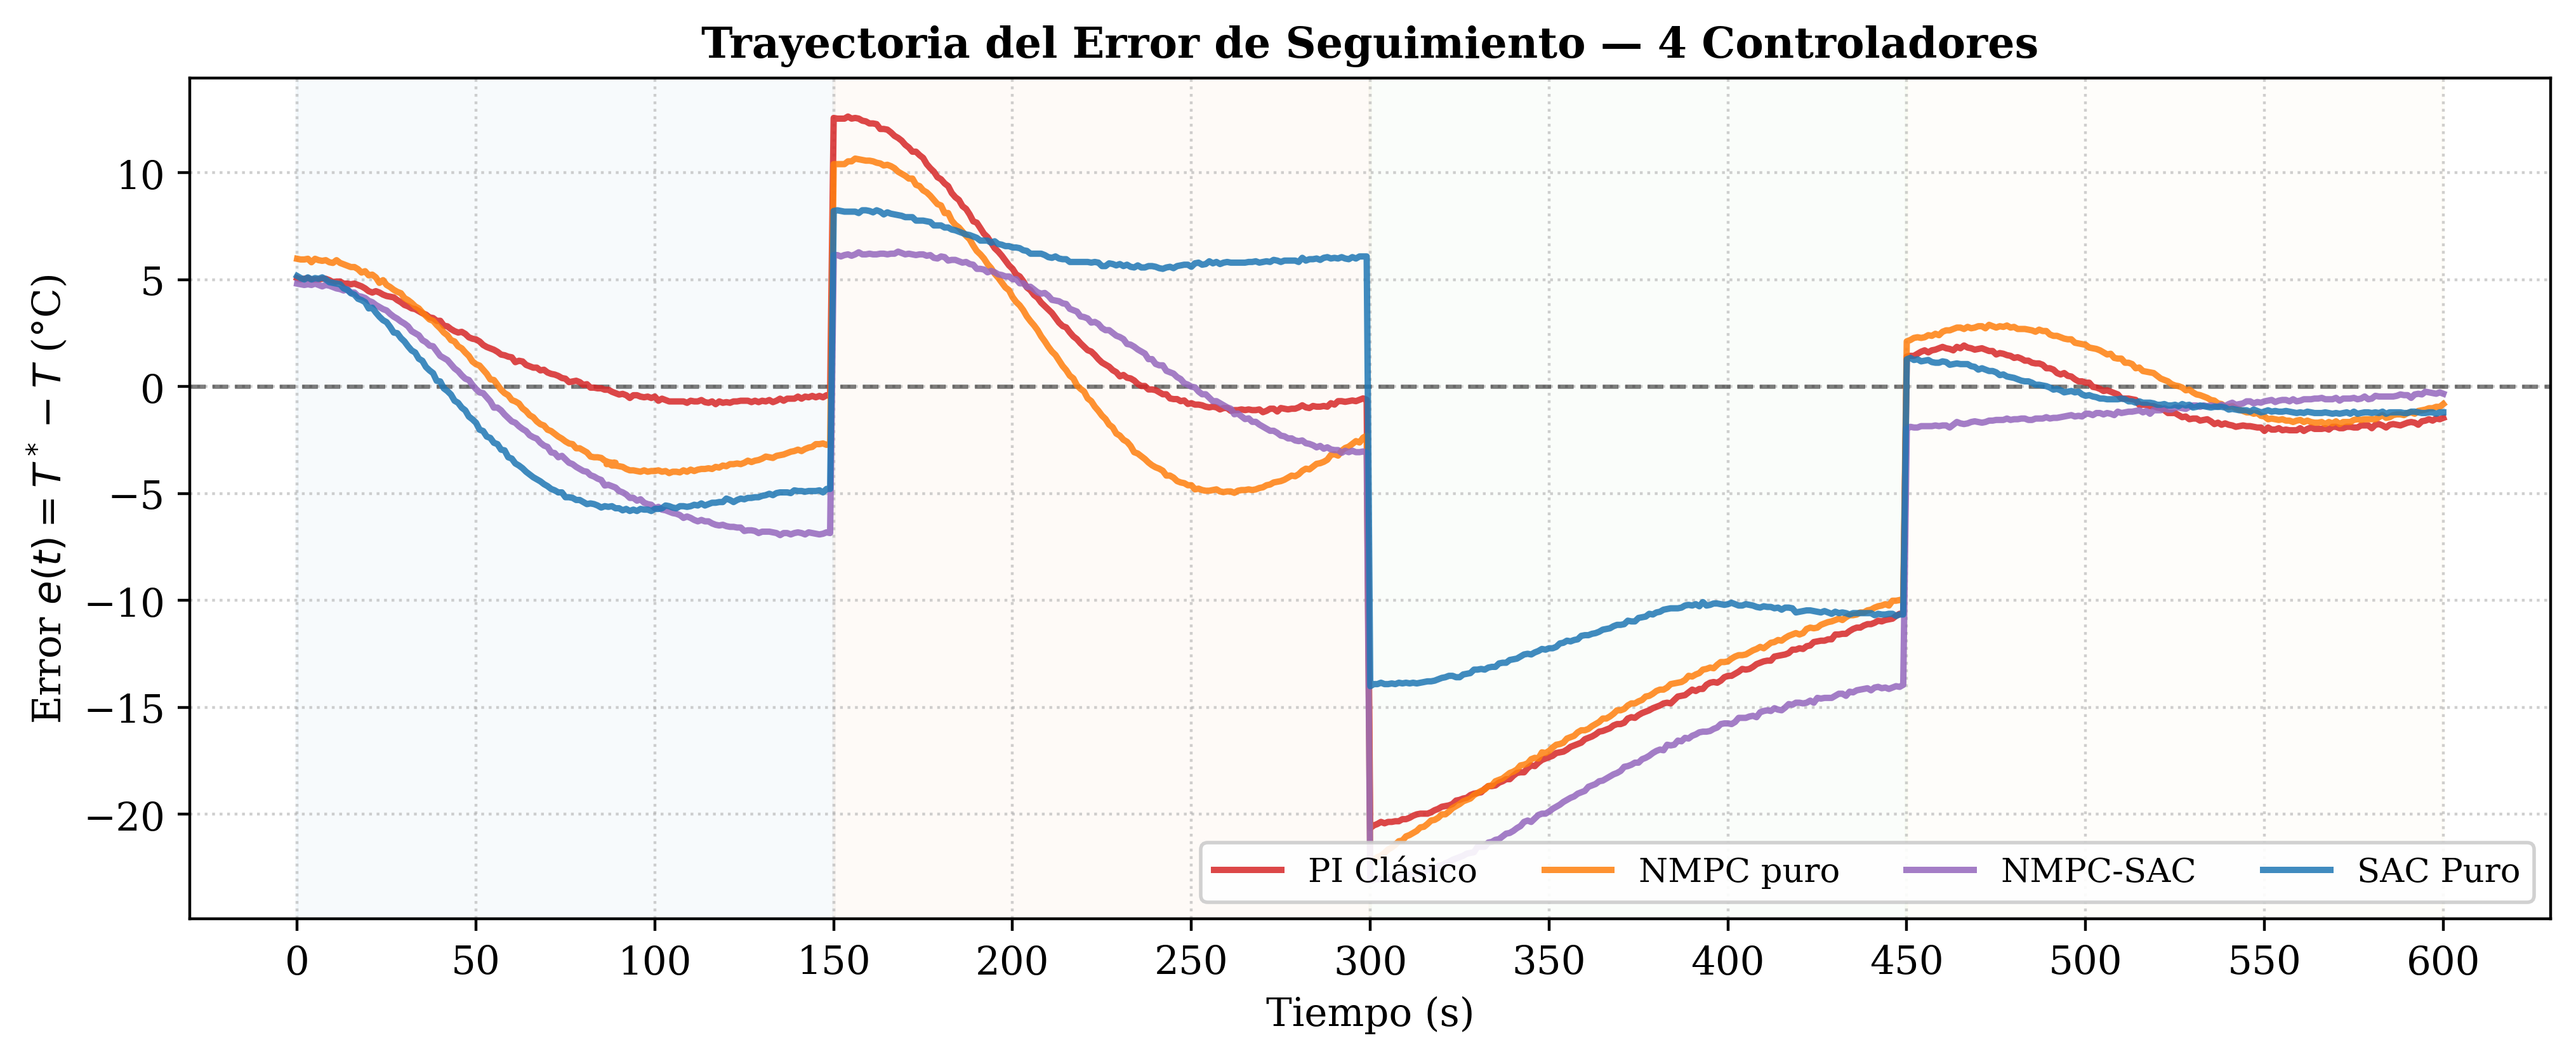
\includegraphics[width=\textwidth]{fig2_error_trajectory.png}
  \caption{Error de seguimiento $e(t) = \Tref(t) - T(t)$ de los cuatro
           controladores (réplica representativa).}
  \label{fig:error}
\end{figure}

\begin{figure}[H]
  \centering
  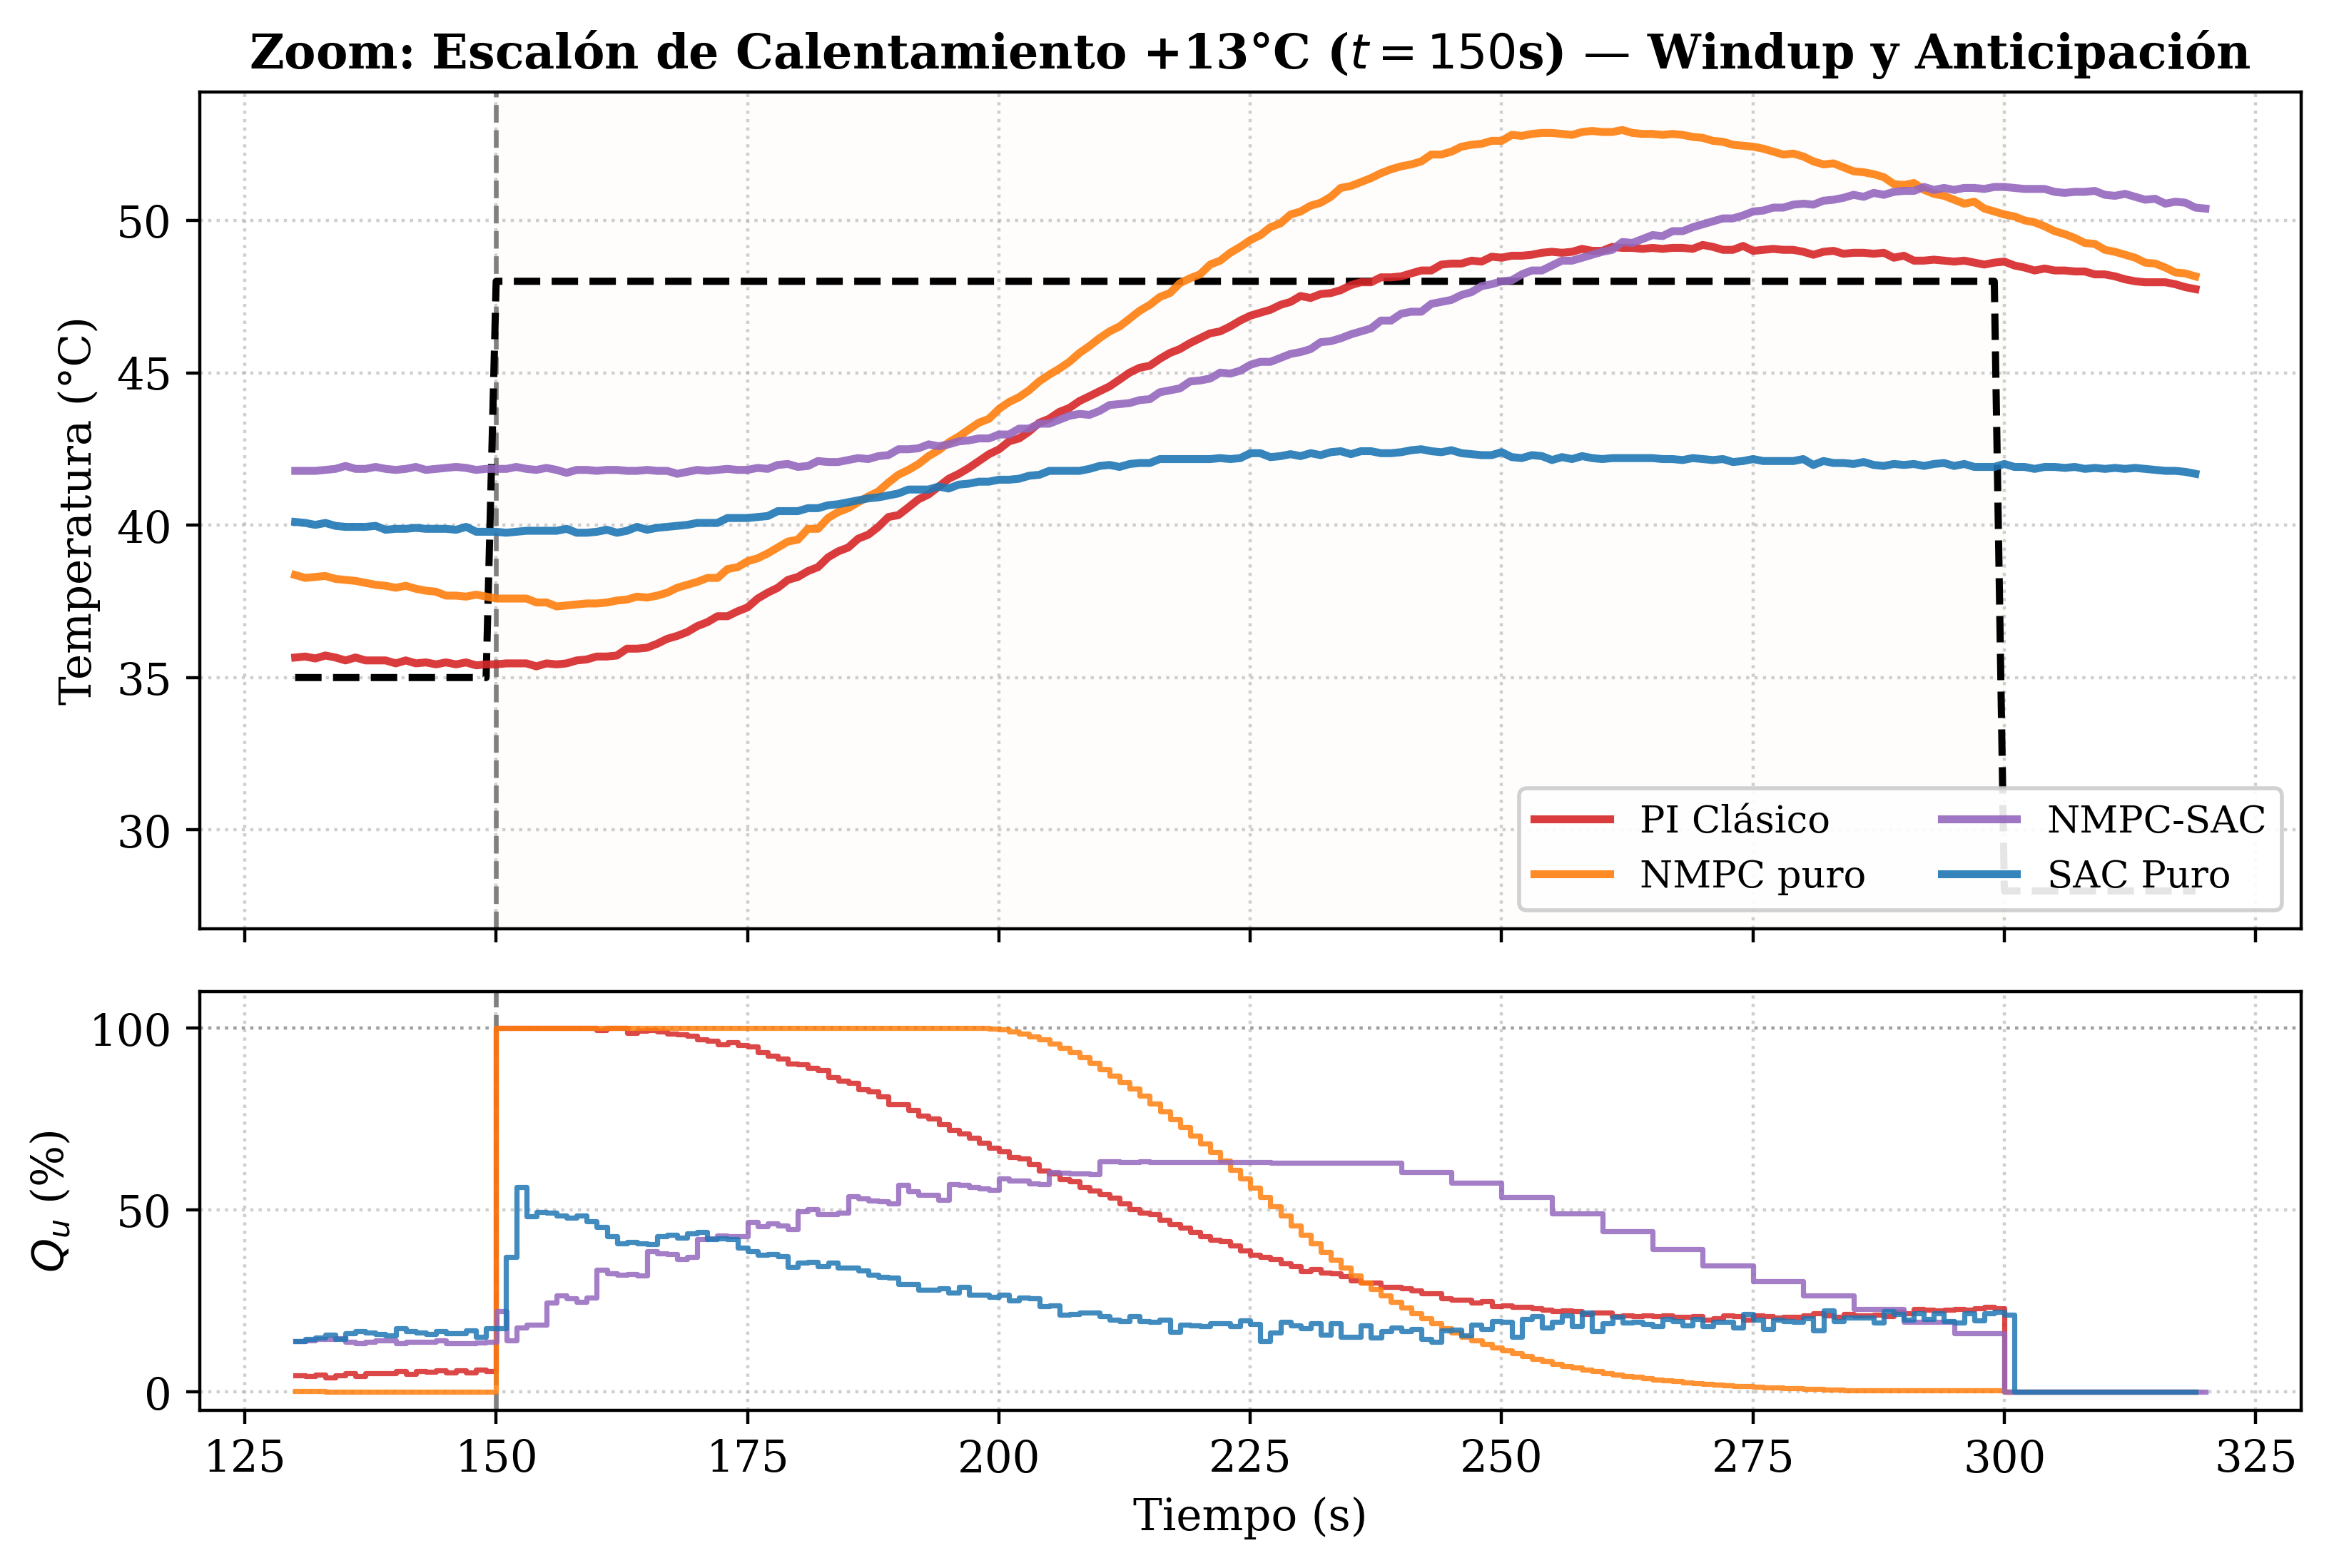
\includegraphics[width=0.92\textwidth]{fig3_zoom_windup.png}
  \caption{Zoom del escalón de calentamiento $+\SI{13}{\celsius}$
           ($t=\SI{150}{\second}$). El SAC anticipa el setpoint y no
           satura; PI y NMPC saturan en $\Qu = 100\,\%$.}
  \label{fig:zoom_windup}
\end{figure}

\begin{figure}[H]
  \centering
  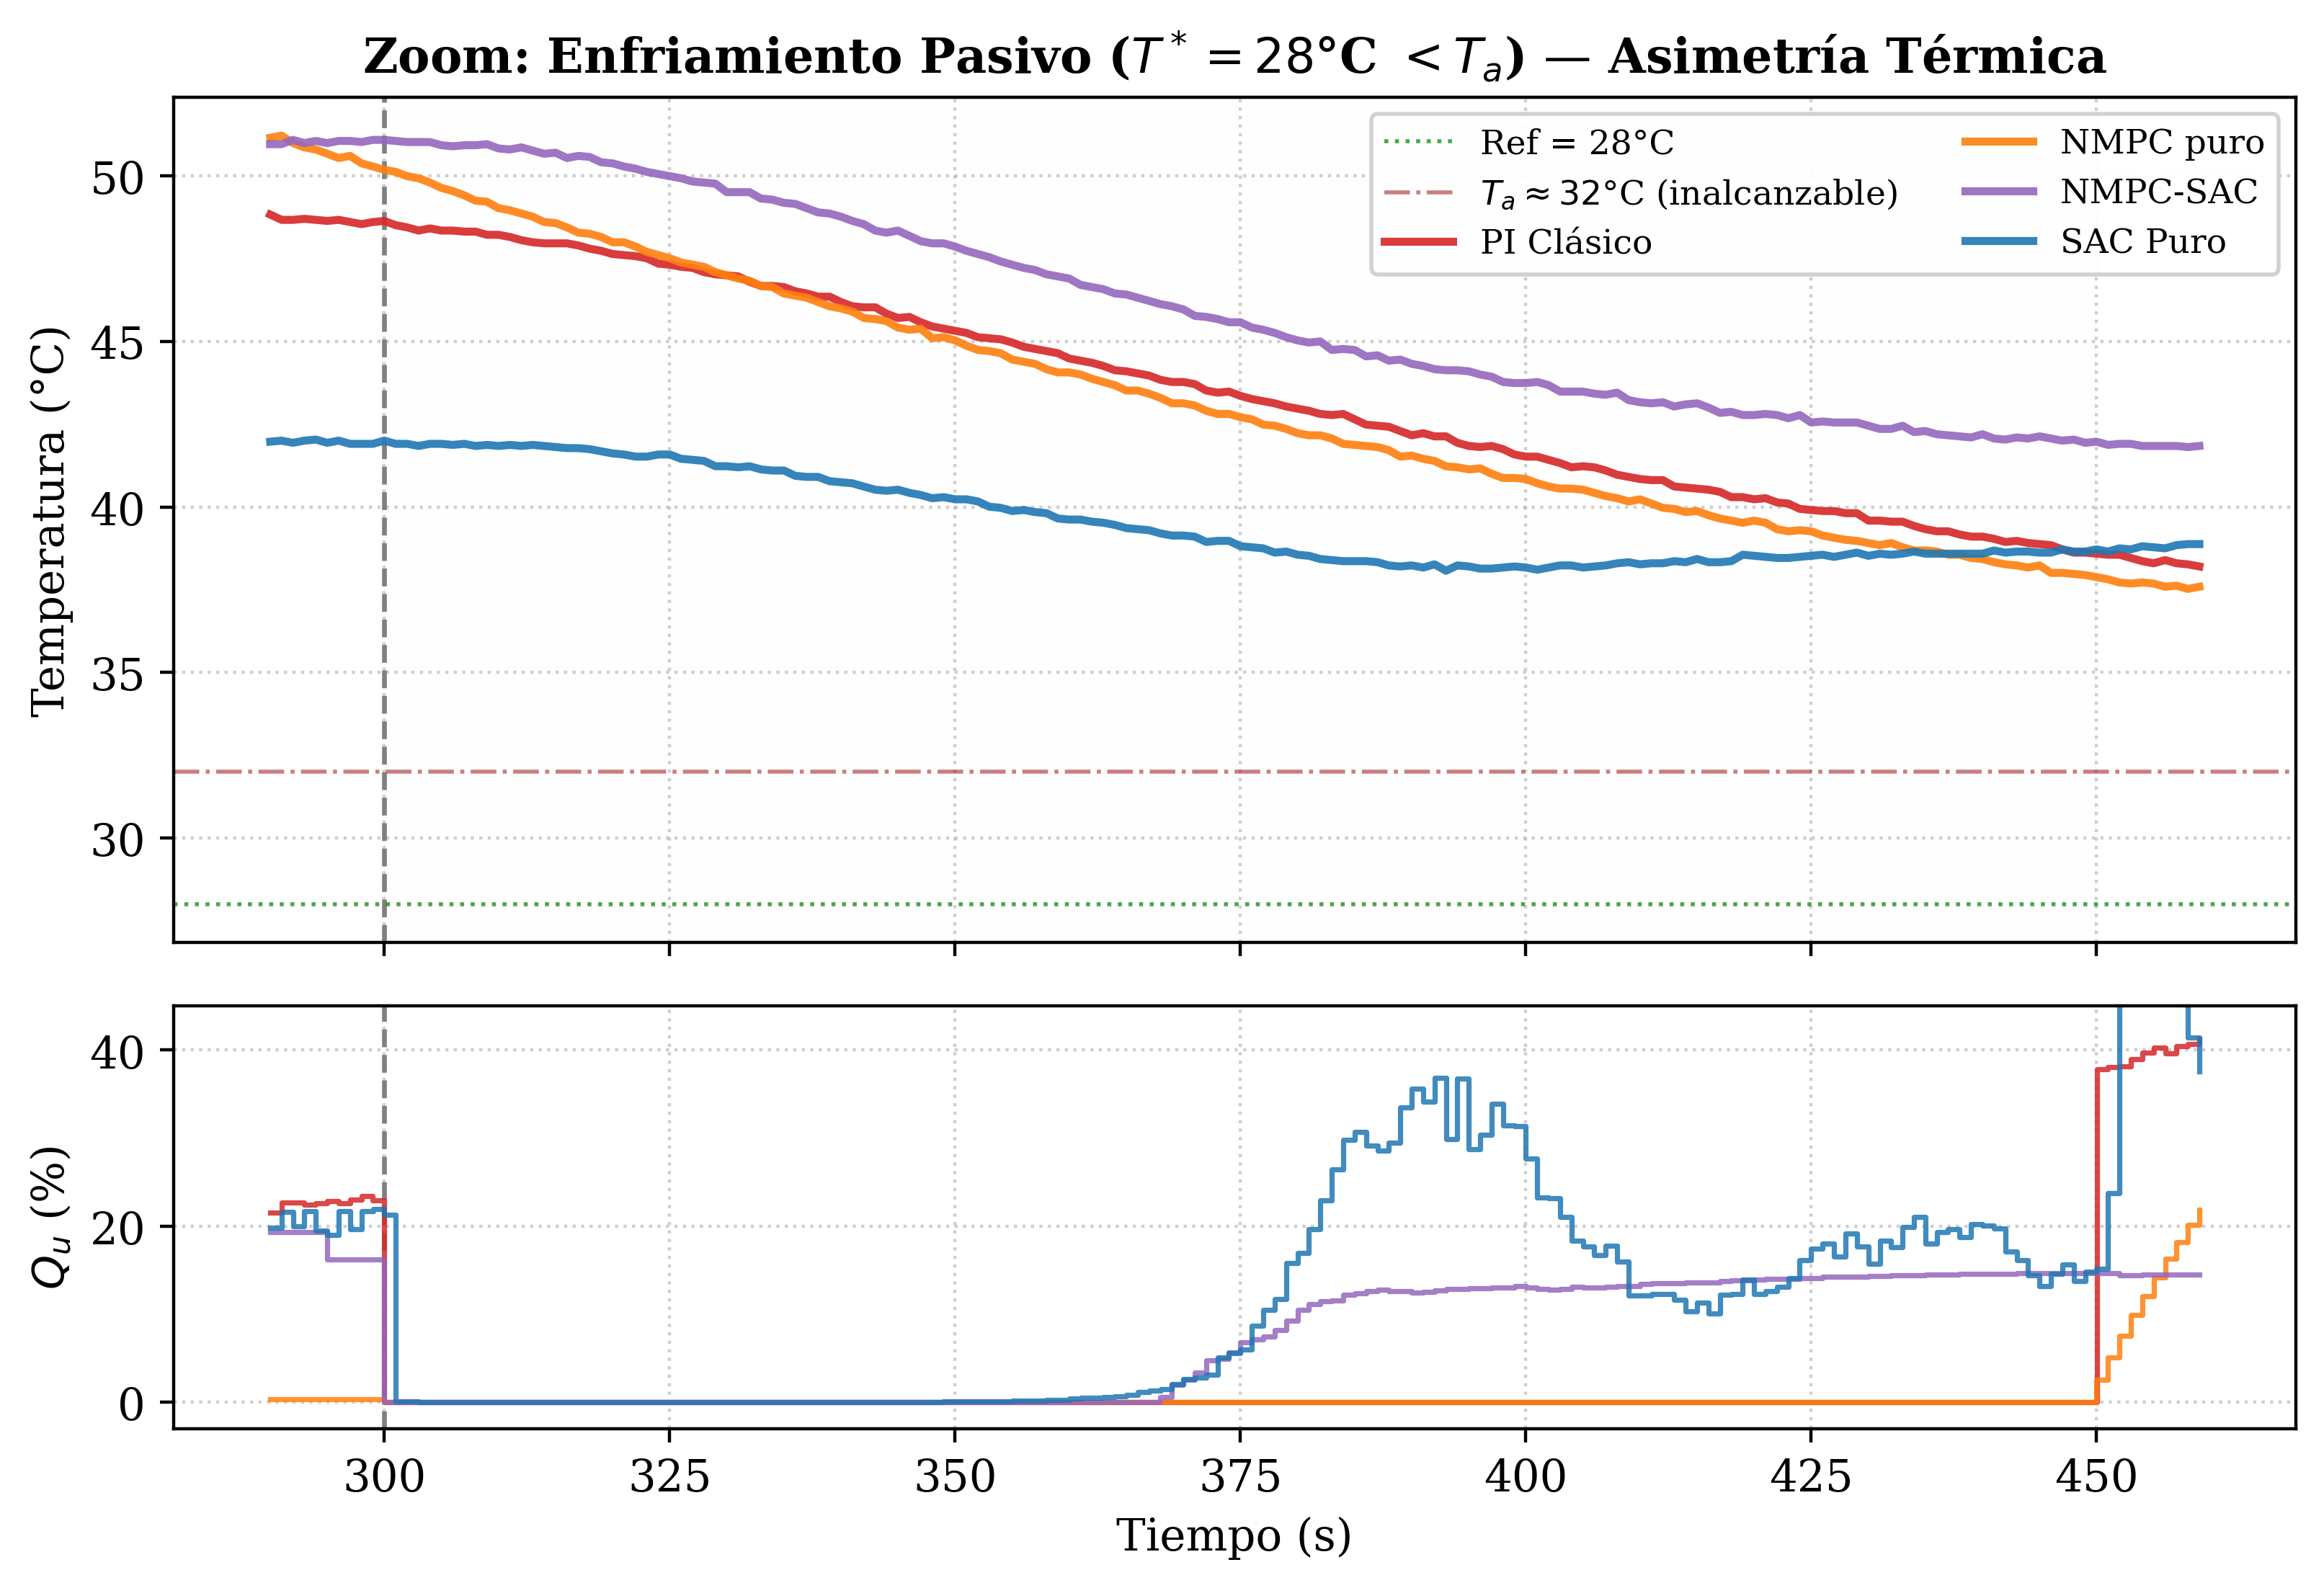
\includegraphics[width=0.92\textwidth]{fig4_zoom_cooling.png}
  \caption{Zoom del enfriamiento pasivo ($\Tref = \SI{28}{\celsius} < T_a$).
           Ningún controlador alcanza el setpoint, pero el SAC llega más cerca
           por entrar a la fase con menor temperatura.}
  \label{fig:zoom_cooling}
\end{figure}

\begin{figure}[H]
  \centering
  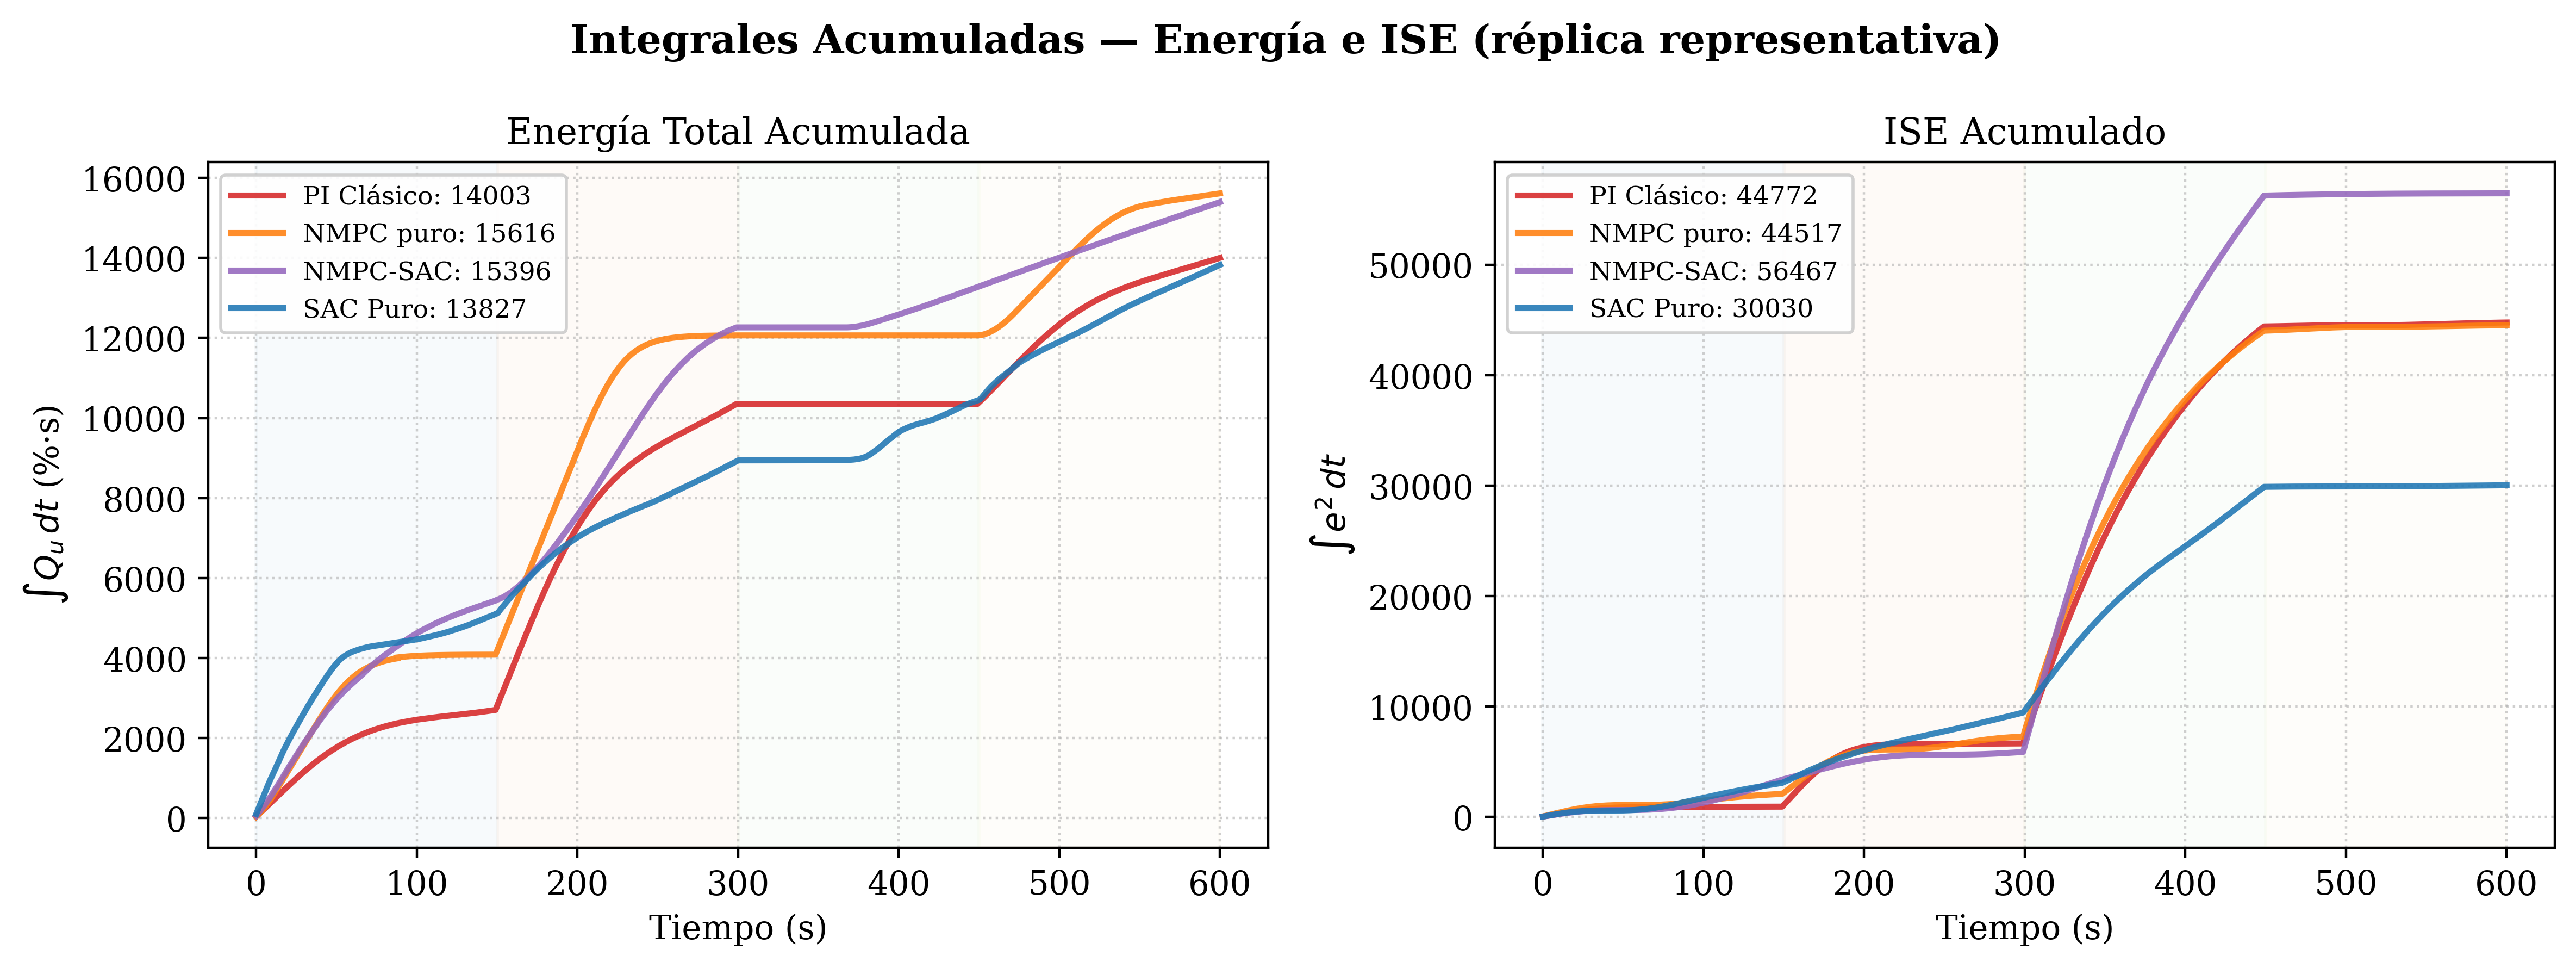
\includegraphics[width=\textwidth]{fig6_integrals.png}
  \caption{Integrales acumuladas de energía (izquierda) e ISE (derecha).
           La mayor divergencia del ISE ocurre en la Fase~3 por el efecto
           de memoria térmica.}
  \label{fig:integrals}
\end{figure}


% =====================================================================
\section{Discusión}
\label{sec:discussion}
% =====================================================================

\subsection{Mecanismo de Windup y Memoria Térmica}
\label{subsec:disc_windup}

Durante el escalón de la Fase~2, el PI satura ($\Qu = 100\,\%$) durante
$\approx\!\SI{16}{\second}$. El término integral acumula, en ese intervalo,
un excedente:

\begin{equation}
  \label{eq:windup_analysis}
  I_{\mathrm{sat}} \approx \bar{e}\, t_{\mathrm{sat}}
  \approx 6.5\,\text{°C} \times 16\,\text{s} = 104\,\text{°C}\cdot\text{s}
\end{equation}

con $\bar{e}$ el error medio durante la saturación. Al cruzar el setpoint,
este excedente produce un impulso adicional
$\Delta\Qu = K_c I_{\mathrm{sat}}/\tau_I = 7.3 \times 104/160.3 \approx
4.7\,\%$, responsable del sobreimpulso modesto ($\SI{1.19}{\celsius}$) del
PI en la Fase~2. Sin embargo, el factor dominante del mal desempeño del PI no es
este overshoot directo, sino la \textbf{memoria térmica}: el anti-windup
condicional opera reactivamente y no puede prevenir que el PI permanezca
caliente al entrar a la Fase~3. PI, NMPC y NMPC-SAC ingresan a la fase de
enfriamiento a $48.7$--$\SI{51.1}{\celsius}$, mientras el SAC lo hace a
$\SI{42.0}{\celsius}$. Como el enfriamiento es exclusivamente pasivo
(Sección~\ref{subsec:disc_cooling}), esta diferencia de $\sim\!\SI{7}{\celsius}$
se traduce en un error cuadrático persistentemente mayor que explica la
divergencia del ISE acumulado (Figura~\ref{fig:integrals}).

\subsection{Causalidad Temporal y Anticipación del SAC}
\label{subsec:disc_causal}

El SAC aventaja a los demás controladores en las Fases~2--4 porque aprende a
lidiar con el retardo del sistema. La temperatura que se mide en $t$
corresponde a la energía inyectada en $t - \theta$, y el historial de 25
acciones previas, que cubre el tiempo muerto nominal de la planta
($25 > \theta = \SI{22.19}{\second}$, en pasos), le permite estimar el estado
real más allá del retardo. El efecto se ve en los números: en la Fase~2 el SAC
mantiene su $\Qu$ máximo en $56.3\,\%$, frente al $100\,\%$ del PI y del NMPC,
y baja la potencia antes de llegar al setpoint porque el historial le indica
que la temperatura real ya está subiendo. Por eso no sobrepasa en la Fase~2.

El sobreimpulso de la Fase~1 ($\SI{5.81}{\celsius}$, superior al del PI)
responde a esa misma lógica pero al revés. Al arrancar, el historial está en
cero y el agente, sin información del retardo, aplica la política de alta
energía que aprendió para los escalones grandes y llega de forma transitoria
a $\Qu = 99.9\,\%$. Es una debilidad de arranque en frío de
la política, mitigable inicializando el historial con el esfuerzo esperado
para el setpoint (Sección~\ref{subsec:future}).

\subsection{Por Qué el NMPC y el NMPC-SAC No Superan al SAC}
\label{subsec:disc_nmpc}

Los datos de hardware de los cuatro controladores permiten un diagnóstico
cuantitativo del resultado. El NMPC puro, pese a usar el
modelo no lineal completo y un horizonte $T_p > \theta$, no supera al PI en
ISE ($44{,}557$ vs.\ $44{,}650$) y lo empeora en sobreimpulso
($\SI{22.2}{\celsius}$ vs.\ $\SI{20.5}{\celsius}$) y energía. La razón es
que el NMPC, al usar parámetros nominales, no compensa el Domain
Randomization real de la planta, y su horizonte finito ($T_p =
\SI{30}{\second}$) es corto frente a la constante de tiempo
($\tau = \SI{179}{\second}$): el NMPC ``ve'' solo una fracción del transitorio
y satura igual que el PI en el escalón grande.

El NMPC-SAC residual es el peor de los cuatro (ISE $55{,}493$,
$+24\,\%$ sobre el NMPC puro). Esto confirma empíricamente los dos
mecanismos de la Sección~\ref{subsec:hybrid}: la restricción
$|\Delta Q| \leq 15\,\%$ impide al agente corregir el comportamiento
conservador del NMPC en la región de alta energía, y el efecto escalera del
solver cacheado introduce excitaciones que degradan el seguimiento. El SAC
puro, libre de ambas restricciones, opera en todo el rango $[0,100]\,\%$ a
\SI{1}{\hertz} sin cacheo, lo que le permite la anticipación que ninguna de
las arquitecturas basadas en modelo logra.

\subsection{Ruido del ADC y Robustez Natural del SAC}
\label{subsec:disc_adc}

El PI responde proporcionalmente al ruido de cuantización:
$\Delta Q_{u,\mathrm{PI}}^{\mathrm{ADC}} = K_c \Delta T_{\mathrm{ADC}} =
7.3 \times 0.097 \approx 0.71\,\%$ por paso. La desviación estándar de
$\Qu$ del PI en estado cuasi-estacionario ($t \in [50,145]$\,s) es
$\sigma_{\Qu,\mathrm{PI}} = 6.24\,\%$ y la del SAC es $8.44\,\%$. La mayor
variabilidad del SAC no proviene de reaccionar al ruido, sino de la
naturaleza estocástica de su política, que realiza una forma de inferencia
probabilística implícita sobre el estado real de la planta, sin requerir un
Filtro de Kalman explícito.

\subsection{Asimetría del Enfriamiento y Restricción Unilateral}
\label{subsec:disc_cooling}

La Fase~3 expone la restricción física fundamental: el actuador solo
calienta ($\Qu \geq 0$). Para $\Qu = 0$:

\begin{equation}
  \label{eq:passive_cooling}
  \frac{dT}{dt}\bigg|_{\Qu = 0}
  = \frac{U_h A (T_a - T) + \varepsilon\sigma A (T_a^4 - T^4)}{m c_p}
\end{equation}

Para $T > T_a$, $\dot{T} < 0$, pero la tasa decae conforme $T \to T_a$. La
temperatura mínima alcanzable es $T_a$, por lo que $\Tref = \SI{28}{\celsius}
< T_a$ es inalcanzable. La diferencia en sobreimpulso de fase (SAC
$\SI{14.0}{\celsius}$ vs.\ $20.7$--$\SI{23.1}{\celsius}$ de los otros) no
refleja diferencias de política durante la Fase~3 (todos tienden a
$\Qu = 0$), sino la memoria térmica: el integrador del PI y el coste del NMPC
``colapsan'' al no poder generar acción negativa, condenando a estos
controladores a esperar la disipación pasiva desde una temperatura más alta.

\subsection{Trade-off: Chattering vs.\ Eficiencia Energética}
\label{subsec:disc_chattering}

El SAC presenta la mayor TV ($725$, frente a $302$--$392$ de los otros) y, a
la vez, el menor consumo energético ($13{,}746$\,\%$\cdot$s). La paradoja se
aclara al mirar qué tipo de variación produce cada controlador. El PI y el
NMPC hacen pocas variaciones de gran amplitud (saturan a $\Qu=100\,\%$ y luego
caen de golpe), que integran mucha energía. El SAC hace muchas variaciones de
pequeña amplitud (chattering de $\pm 3$--$8\,\%$) en torno a un punto de
operación más bajo, y por eso consume menos. La
Figura~\ref{fig:chattering} cuantifica esta diferencia en el estado
cuasi-estacionario. Desde la perspectiva de la vida útil del actuador, el
chattering de baja amplitud es menos perjudicial que la saturación
prolongada \cite{Astrom2006}.

\begin{figure}[H]
  \centering
  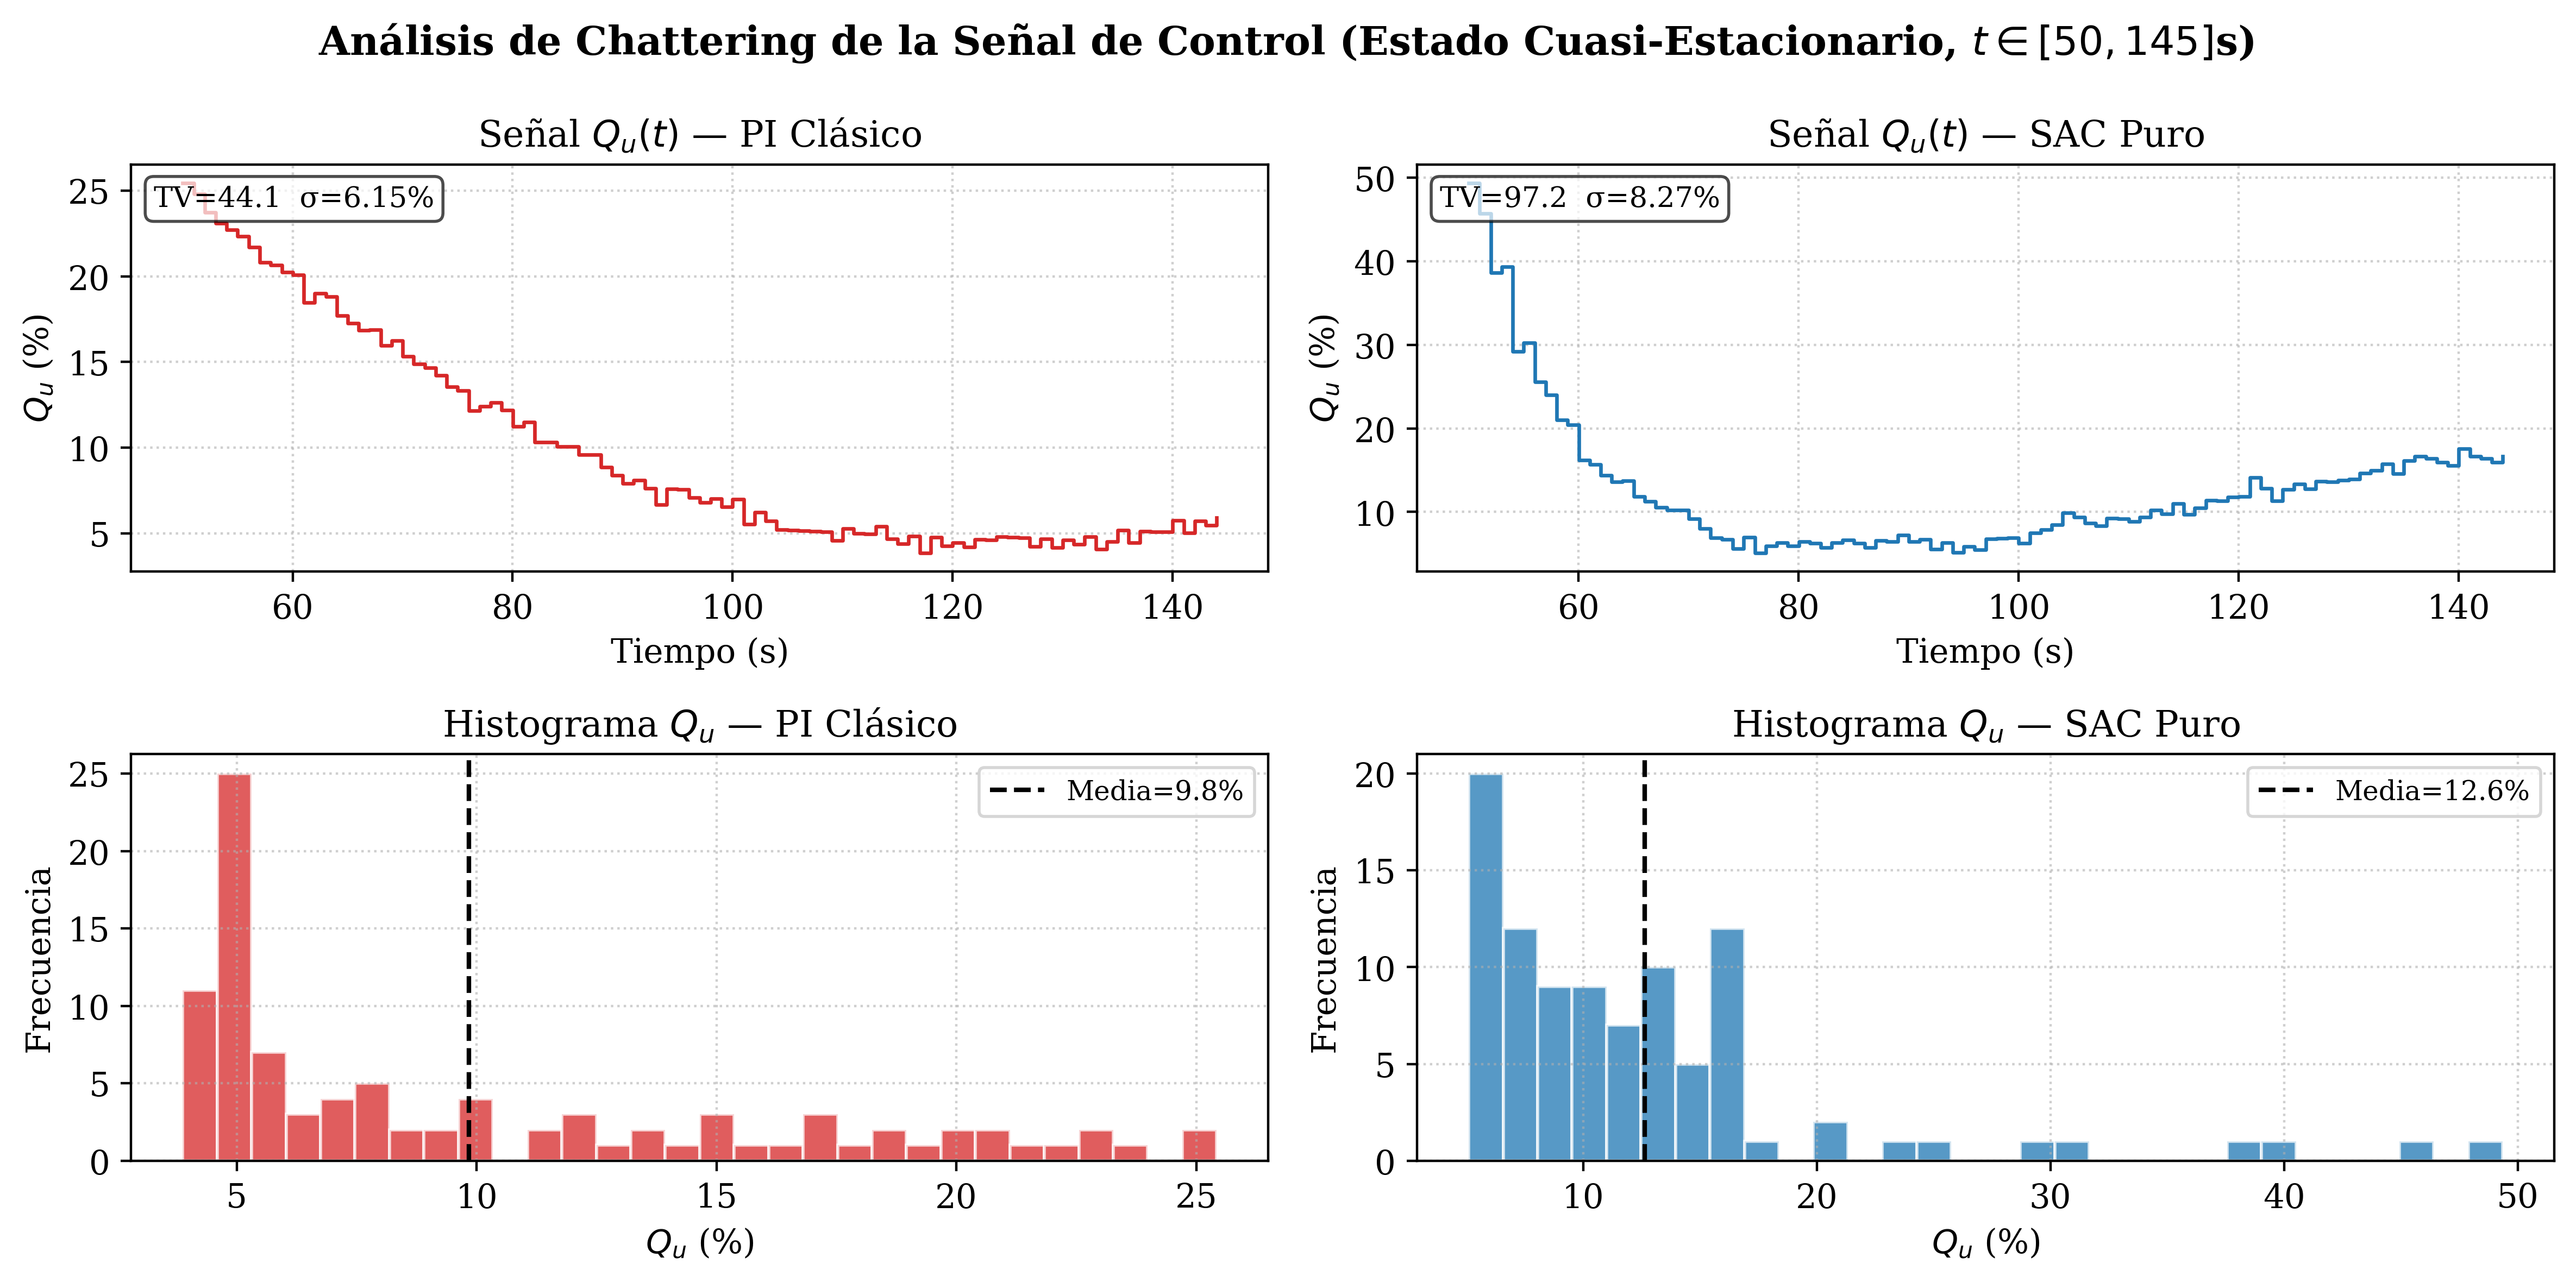
\includegraphics[width=\textwidth]{fig5_chattering_analysis.png}
  \caption{Análisis de chattering en estado cuasi-estacionario
           ($t \in [50,145]$s). El histograma del SAC es más amplio,
           reflejando su política estocástica, pero centrado en un $\Qu$
           medio menor.}
  \label{fig:chattering}
\end{figure}

\subsection{Limitaciones y Trabajo Futuro}
\label{subsec:future}

\begin{enumerate}
  \item \textbf{Sobreimpulso de arranque en frío.} La inicialización del
  historial a cero produce overshoot inicial de $\SI{5.81}{\celsius}$ en la
  Fase~1. Solución: inicializar el historial con el $\Qu$ esperado para el
  setpoint.
  \item \textbf{Reducción del chattering.} Un término de suavizado
  $-\lambda_{\mathrm{TV}}|\Delta\Qu|$ en la recompensa reduciría la TV, a
  costa de la agresividad de respuesta.
  \item \textbf{Validación multi-dispositivo.} Las réplicas se obtuvieron
  sobre un único dispositivo TCLab. La validación cruzada sobre 3--5
  unidades en distintas condiciones ambientales reforzaría la
  generalización.
  \item \textbf{Comparación con TD3 bajo idénticas condiciones.} La
  comparación directa con un agente TD3 entrenado con el mismo Curriculum se
  identifica como trabajo futuro para aislar el aporte de la regularización
  por entropía del SAC.
\end{enumerate}


% =====================================================================
\section{Conclusiones}
\label{sec:conclusions}
% =====================================================================

Este artículo comparó cuatro esquemas de control de temperatura (PI
clásico, NMPC puro, arquitectura híbrida residual NMPC-SAC y SAC puro) en
hardware real (TCLab Arduino) bajo un perfil de estrés dinámico de cuatro
fases asimétricas, con cuatro réplicas por controlador y análisis de
significancia estadística. El agente SAC, entrenado mediante Curriculum
Learning de cuatro etapas con tiempos muertos dinámicos de hasta
\SI{33}{\second} y Domain Randomization de $\pm 15\,\%$, redujo el ISE en un
$32.5\,\%$ respecto al PI y en un $32.4\,\%$ respecto al NMPC, con un
sobreimpulso máximo de $\SI{14.0}{\celsius}$ frente a $20.5$--$\SI{22.9}{\celsius}$
de las alternativas. La superioridad en ISE es estadísticamente
significativa (Mann-Whitney, $p = 0.0143$).

La ventaja del SAC se debe a su manejo del tiempo muerto. Como la observación
incluye el historial de acciones, el agente infiere el estado real de la
planta pese al retardo y reduce la potencia antes de que la temperatura
alcance el setpoint, con lo que evita la saturación y el windup que la
acompaña. El agente aprende este comportamiento anticipativo durante el
entrenamiento, sin un modelo explícito de la planta.

La comparación cuantitativa de los cuatro controladores deja tres resultados
metodológicos. El primero es que el NMPC puro no supera al PI en este escenario
severo, porque su horizonte finito y su dependencia de parámetros nominales le
impiden anticipar mejor que el SAC. El análisis de sensibilidad confirma además
que ni una resintonización específica del NMPC cierra la brecha con el SAC
(Sección~\ref{subsec:nmpc_sensitivity}). El segundo es que la arquitectura
híbrida NMPC-SAC resultó la peor de las cuatro, porque la restricción de su
espacio de exploración y el efecto escalera de su base cacheada degradan el
desempeño por debajo del NMPC puro. La hibridación modelo-basado/modelo-libre,
por tanto, no garantiza mejoras y puede ser contraproducente en hardware con
ruido de ADC y restricciones de cómputo. El tercero, de valor para la
metodología de entrenamiento, es que el orden de desempeño obtenido en
simulación (SAC $<$ PI $<$ NMPC $<$ NMPC-SAC en ISE) se conserva íntegramente
en hardware (Tabla~\ref{tab:metricas_sim} frente a la
Sección~\ref{subsec:dyn_stress}), lo que valida el simulador ODE empleado para
entrenar el agente y respalda su transferencia directa a la planta real sin
reentrenamiento.

El SAC tiene dos contrapartidas. Una es una Variación Total mayor, debida a un
chattering de baja amplitud que compensa con un menor consumo de energía. La
otra es un desempeño algo inferior en regulación a setpoint constante, justo
el escenario para el que se diseñó el PI. El SAC marca la diferencia en las
condiciones que más cuestan a los métodos clásicos y predictivos: escalones
grandes, tiempos muertos largos, ruido de sensor y enfriamiento asimétrico. En
conjunto, los resultados muestran que un agente de aprendizaje por refuerzo
profundo entrenado en simulación con Domain Randomization y Curriculum Learning
puede igualar y superar al control clásico y predictivo en control térmico
severo. Su extrapolación a plantas industriales de mayor escala exige
validación en varias unidades y bajo condiciones ambientales variables.


% =====================================================================
% ── METADATOS DE CIERRE ─────────────────────────────────────────────
% =====================================================================
% Bloques de metadatos propios del envío a revista MDPI. En una monografía
% imprimen etiquetas en inglés sin contenido, por lo que se omiten. Para
% reactivar Agradecimientos o Financiación, descoméntese y rellénese en español.
% \authorcontributions{ }
% \funding{ }
% \dataavailability{ }
% \acknowledgments{ }
% \conflictsofinterest{ }

\abbreviations{Abreviaturas}{%
\noindent
\begin{tabular}{@{}ll}
ADC  & Conversor Analógico-Digital \\
CL   & \textit{Curriculum Learning} \\
DDPG & \textit{Deep Deterministic Policy Gradient} \\
DR   & \textit{Domain Randomization} \\
DRL  & Aprendizaje por Refuerzo Profundo \\
FOPDT & Primer Orden con Tiempo Muerto \\
IAE  & Error Absoluto Integral \\
IMC  & Control por Modelo Interno \\
ISE  & Error Integral Cuadrático \\
ITAE & Error Absoluto Integral Ponderado en el Tiempo \\
NMPC & Control Predictivo No Lineal \\
ODE  & Ecuación Diferencial Ordinaria \\
PI   & Proporcional-Integral \\
SAC  & \textit{Soft Actor-Critic} \\
SLSQP & \textit{Sequential Least Squares Programming} \\
SP   & Predictor de Smith \\
TCLab & \textit{Temperature Control Lab} \\
TD3  & \textit{Twin Delayed Deep Deterministic Policy Gradient} \\
TV   & Variación Total \\
\end{tabular}}

% =====================================================================
% ── REFERENCIAS ─────────────────────────────────────────────────────
% =====================================================================
\begin{thebibliography}{99}

\bibitem{Seborg2016}
Seborg, D.E.; Edgar, T.F.; Mellichamp, D.A.; Doyle, F.J., III.
\textit{Process Dynamics and Control}, 4th ed.;
Wiley: Hoboken, NJ, USA, 2016.

\bibitem{Astrom2006}
Åström, K.J.; Hägglund, T.
\textit{Advanced PID Control};
ISA: Research Triangle Park, NC, USA, 2006.

\bibitem{Skogestad2003}
Skogestad, S.
Simple Analytic Rules for Model Reduction and PID Controller Tuning.
\textit{J.\ Process Control} \textbf{2003}, \textit{13}, 291--309.

\bibitem{Smith1957}
Smith, O.J.M.
Closed Control of Loops with Dead Time.
\textit{Chem.\ Eng.\ Prog.} \textbf{1957}, \textit{53}, 217--219.

\bibitem{NormeyRico2007}
Normey-Rico, J.E.; Camacho, E.F.
\textit{Control of Dead-Time Processes};
Springer: London, UK, 2007.

\bibitem{Hedengren2019}
Hedengren, J.D.; Martin, R.A.; Nash, A.; Forrest, B.
TCLab Temperature Control Laboratory.
\textit{Processes} \textbf{2019}, \textit{7}, 130.
\doi{10.3390/pr7030130}

\bibitem{Park2020}
Park, J.; Martin, R.A.; Kelly, J.D.; Hedengren, J.D.
Benchmark Temperature Microcontroller for Process Dynamics and Control.
\textit{Comput.\ Chem.\ Eng.} \textbf{2020}, \textit{135}, 106736.

\bibitem{Rawlings2017}
Rawlings, J.B.; Mayne, D.Q.; Diehl, M.
\textit{Model Predictive Control: Theory, Computation, and Design},
2nd ed.; Nob Hill Publishing: Madison, WI, USA, 2017.

\bibitem{Mayne2014}
Mayne, D.Q.
Model Predictive Control: Recent Developments and Future Promise.
\textit{Automatica} \textbf{2014}, \textit{50}, 2967--2986.

\bibitem{SozaMamani2025}
Soza Mamani, K.M.; Prado Romo, A.J.
Integrating Model Predictive Control with Deep Reinforcement Learning for
Robust Control of Thermal Processes with Long Time Delays.
\textit{Processes} \textbf{2025}, \textit{13}, 1627.
\doi{10.3390/pr13061627}

\bibitem{Sutton2018}
Sutton, R.S.; Barto, A.G.
\textit{Reinforcement Learning: An Introduction}, 2nd ed.;
MIT Press: Cambridge, MA, USA, 2018.

\bibitem{Mnih2015}
Mnih, V.; et al.
Human-Level Control through Deep Reinforcement Learning.
\textit{Nature} \textbf{2015}, \textit{518}, 529--533.

\bibitem{Lillicrap2016}
Lillicrap, T.P.; Hunt, J.J.; Pritzel, A.; Heess, N.; Erez, T.; Tassa, Y.;
Silver, D.; Wierstra, D.
Continuous Control with Deep Reinforcement Learning.
In \textit{Proc.\ ICLR 2016}, San Juan, Puerto Rico, 2--4 May 2016.

\bibitem{Fujimoto2018}
Fujimoto, S.; van Hoof, H.; Meger, D.
Addressing Function Approximation Error in Actor-Critic Methods.
In \textit{Proc.\ 35th Int.\ Conf.\ Mach.\ Learn.\ (ICML)},
Stockholm, Sweden, 10--15 July 2018; Vol.~80, pp.~1587--1596.

\bibitem{Rajasekhar2023}
Rajasekhar, N.; Radhakrishnan, T.K.; Samsudeen, N.
RL--DDPG Based Temperature Control of Fermentation Bioreactor for Ethanol
Production.
In \textit{Proc.\ Int.\ Conf.\ Exhib.\ Sustain.\ Chem.\ Eng.},
Mumbai, India, 14--16 September 2023.

\bibitem{Joshi2021}
Joshi, T.; Makker, S.; Kodamana, H.; Kandath, H.
Application of Twin Delayed Deep Deterministic Policy Gradient Learning for
the Control of Transesterification Process.
\textit{arXiv} \textbf{2021}, arXiv:2102.13012.

\bibitem{Spielberg2019}
Spielberg, S.P.K.; Gopaluni, R.B.; Loewen, P.D.
Deep Reinforcement Learning Approaches for Process Control.
In \textit{Proc.\ 6th IFAC Conf.\ NMPC}, Madison, WI, USA, 2019;
Vol.~52, pp.~567--572.

\bibitem{Dogru2022}
Dogru, O.; Velswamy, K.; Ibrahim, F.; Wu, Y.; Sundaramoorthy, A.S.;
Huang, B.; Xu, S.; Nixon, M.; Bell, N.
Reinforcement Learning Approach to Autonomous PID Tuning.
\textit{Comput.\ Chem.\ Eng.} \textbf{2022}, \textit{161}, 107760.

\bibitem{Haarnoja2018}
Haarnoja, T.; Zhou, A.; Abbeel, P.; Levine, S.
Soft Actor-Critic: Off-Policy Maximum Entropy Deep Reinforcement Learning
with a Stochastic Actor.
In \textit{Proc.\ 35th Int.\ Conf.\ Mach.\ Learn.\ (ICML)},
Stockholm, Sweden, 10--15 July 2018; Vol.~80, pp.~1861--1870.

\bibitem{Bengio2009}
Bengio, Y.; Louradour, J.; Collobert, R.; Weston, J.
Curriculum Learning.
In \textit{Proc.\ 26th Int.\ Conf.\ Mach.\ Learn.\ (ICML)},
Montreal, Canada, 14--18 June 2009; pp.~41--48.

\bibitem{Narvekar2020}
Narvekar, S.; Peng, B.; Leonetti, M.; Sinapov, J.; Taylor, M.E.; Stone, P.
Curriculum Learning for Reinforcement Learning Domains: A Framework
and Survey.
\textit{J.\ Mach.\ Learn.\ Res.} \textbf{2020}, \textit{21}, 181.

\bibitem{Hosseinionari2024}
Hosseinionari, H.; Seethaler, R.
The Integration of Model Predictive Control and Deep Reinforcement Learning
for Efficient Thermal Control in Thermoforming Processes.
\textit{J.\ Manuf.\ Process.} \textbf{2024}, \textit{115}, 82--93.

\bibitem{Chen2022}
Chen, L.; Meng, F.; Zhang, Y.
An HVAC Control Approach via Combining Model-Based Deep Reinforcement
Learning and Model Predictive Control.
\textit{IEEE Internet Things J.} \textbf{2022}, \textit{9}, 19160--19173.

\bibitem{Raffin2021}
Raffin, A.; Hill, A.; Gleave, A.; Kanervisto, A.; Ernestus, M.; Dormann, N.
Stable-Baselines3: Reliable Reinforcement Learning Implementations.
\textit{J.\ Mach.\ Learn.\ Res.} \textbf{2021}, \textit{22}, 268.

\end{thebibliography}

\end{document}
